\documentclass[a4paper,12pt]{amsart}

\input preambolo

\renewcommand{\textbf}[1]{\text{\fontseries{b}\selectfont{\upshape #1}}}

\newcommand{\pullback}[2]{\node at ($(#1)!.2!(#2)$) {$\lrcorner$}}
\newcommand{\pushout}[2]{\node  at ($(#1)!.8!(#2)$) {$\ulcorner$}}
\newcommand{\pullout}[2]{\pullback{#1}{#2}; \pushout{#1}{#2}}

% \usepackage[usenames,dvipsnames]{xcolor}
  \definecolor{semilightgray}{rgb}{0.65, 0.65, 0.65}
  \def\gray#1{\textcolor{semilightgray}{#1}}

\begin{document}
\title{Hearts and towers in stable $\infty$-categories}
\author{Domenico Fiorenza$^\dag$, Fosco Loregi\`an$^\ddag$}
	\address{%
	\textsf{Domenico Fiorenza}: 
	Dipartimento di Matematica ``Guido Castelnuovo'', 
	Universit\`a degli Studi di Roma ``la Sapienza'',	
	P.le Aldo Moro 2 -- \oldstylenums{00185} -- Roma. 
	}

	\email{\href{mailto:fiorenza@mat.uniroma1.it}{\tt fiorenza@mat.uniroma1.it}}
	\email{\href{mailto:floregia@uwo.ca}{\tt floregia@uwo.ca}, \href{mailto:fosco.loregian@gmail.com}{\tt fosco.loregian@gmail.com}}

\date{\today}
\maketitle 

\begin{abstract}
In the present section we exploit the description of $t$-structures as normal torsion theories of our previous \cite{Fiorenza2014} to discuss two apparently separated constructions in the theory of triangulated categories: the characterization of \emph{bounded} $t$-\emph{structures} in terms of their hearts, and \emph{semiorthogonal decompositions} on triangulated categories. In the stable setting both notions stem as particular cases of a single construction. 
\end{abstract}
\section*{Introduction}
The purpose of this brief subsection is to give an account of results and notation from our previous \cite{Fiorenza2014}, of which the present work is a natural follow-up. We borrow from \cite{Fiorenza2014} for all that concerns categories and higher categories, functors, simplicial sets, and in particular the basic theory of quasicategorical factorization systems, $t$-structures on stable $\infty$-categories and related topics. Since the aim of this section is only to provide a reference, statements will be recalled in a sketchy form; we refer the reader to \cite{Fiorenza2014} for a detailed rigorous version of these results.

The starting point is the following rephrasing of \cite[Prop. \textbf{2.2}]{CHK}.
\begin{proposition*}
Let $\C$ be a category with a terminal object. There exists an antitone Galois connection $\Phi\dashv \Psi$ between the poset $\text{Rex}(\C)$ of reflective subcategories of $\C$ and the poset $\textsc{pf}(\C)$ of prefactorization systems on $\C$. The morphism $\Psi$ sends the factorization system $\fF=(\E,\M)$ to the reflexive subcategory $\M/1 = \{B\in\C\mid (B\to 1)\in\M\}$, and $\Phi$ is defined  by sending  a reflective subcategory $\cate{B}$ of $\cate{C}$ to the prefactorization system right generated by $\hom(\cate B)\subseteq \hom(\C)$. 
\end{proposition*}
This is one of the fundamental results in \cite[Thm. \textbf{3.13}]{Fiorenza2014}, asserting that
\begin{theorem*}
Let $\C$ be a stable $\infty$-category. There is a bijective correspondence between the class of normal torsion theories and the class of $t$-structures on $\C$.
\end{theorem*}
\begin{remark*}
The partial order on $\textsc{pf}(\C)$ is given by $\fF_{=(\E,\M)}\preceq \fF'_{= (\E',\M')}$ iff $\M\subset\M'$ (or equivalently, $\E'\subset \E$). We endow the collection of normal torsion theories (and then the collection of $t$-structures on $\C$) with the induced order.
\end{remark*}
Finally, we recall a simple and yet pervasive result in the context of torsion theories in stable $\infty$-categories.
\begin{lemma*}[Sator Lemma]
In a pointed quasicategory $\C$, an initial arrow $0\to A$ lies in a class $\E$ or $\M$ of a bireflective factorization system $\fF$ if and only if the terminal arrow $A\to 0$ lies in the same class.
\end{lemma*}
In analogy with the example of the Postnikov decomposition of a morphism $f\colon X\to Y$ of spaces (or spectra, or objects of an $\infty$-topos), we construct (\adef \refbf{tower.of.f}) the \emph{tower} $\rook_{\{i_j\}}(f)$\footnote{Pron. \emph{rook}; it is the same rook of the game of chess.} of a morphism induced by a $\Z$-equivariant \emph{$J$-family} of normal torsion theories $\{\fF_i\}_{i\in J}$, \ie a monotone function $J \to\fs(\C)$ ``taking normal values'', which is \emph{equivariant} with respect to an action of the group $\Z$ on both sets.

As we will see, a natural way to encompass these structures is to vary the action on the domain of the $J$-family (choosing diffferent $J$s and different actions on $J$ will result in different kinds of $t$-structures for the values $J(\lambda)$. We will concentrate on the following two ``extremal'' examples:
\begin{itemize}
\item For $J=\Z$ with its obvious self-action, we recover the classical notion of Postnikov towers in a triangulated category endowed with a $t$-structure (and a fortiori, the notion of Postnikov tower in the category $\cate{Sp}$ of spectra), and subsequently we give a neat, conceptual proof of the the abelianity of the \emph{heart} of a $t$-structure in the stable setting, basically relying on the uniqueness of a suitable factorization. 

\item For $J$ a finite totally ordered set, or more generally any set $J$ with trivial $\Z$-action, we recover the theory of \emph{semiorthogonal decompositions} \cite{Bondal1995, Kuz}, showing in \athm \refbf{what.s.semiortho} that such a $J\to \fs_\nu(\C)$ consists of a family $\{\fF_i\}_{i\in J}$ of \emph{stable} $t$-structures. This is a classical result.
\end{itemize}
\section{Posets with \texorpdfstring{$\Z$}{Z}-actions.}
\epigraph{\begin{CJK*}{UTF8}{bsmi} 為無為。事無事。味無味。\end{CJK*}}{Laozi \textsc{lxiii}}
This section has an introductory purpose, aiming to introduce the terminology about partially ordered groups and their actions, and then specialize the discussion to $\Z$-actions on partially ordered sets.

We do not aim at reaching a complete generality, but instead at gathering a number of useful results and nomenclature which is useful to have at hand. Among various possible choices, we mention specialized references as \cite{blyth2005lattices, glass1999partially, Fuch63} for an extended discussion of the theory of actions on ordered groups.
\begin{definition}
A \emph{partially ordered group} (``po-group'' for short) consists of a group $\mathbf{G} = (G, \cdot,1)$ endowed with a relation $\preceq$ which is a partial order and a (two-sided) congruence on $G$, namely for any $g\preceq h$ and $a,b\in \mathbf{G}$ we have 
\begin{itemize}
\item[(i)] $a\cdot g\preceq a\cdot h$ and
\item[(ii)] $g\cdot b\preceq h\cdot b$.
\end{itemize}
\end{definition}
\begin{remark}
We should draw a distinction between a \emph{left} po-group (satisfying only property \emph{i} above) and a \emph{right} po-group (satisfying only \emph{ii}). At the level of generality we need ignoring this subtlety is absolutely harmless.

A supplementary motivation to choose this slightly looser definition is that it seems more natural for a group to be ordered by a two-sided congruence, since in this case inversion $(-)^{-1}\colon \cate{G} \to \cate{G}$ is an antitone antiautomorphism of groups, \ie we have that
\begin{itemize}
\item $g\preceq h \iff h^{-1}\preceq g^{-1}$;
\item The set $G^+$ of \emph{positive} elements, i.e. the set $\{g\in G\mid 1\preceq g\}$ is closed under conjugation.
\end{itemize}
\end{remark}
\begin{definition}
A \emph{homomorphism} of po-groups consists of a group morphism $f\colon G\to H$ which is also a monotone mapping. This, with the obvious choices of identities and composition, defines a category $\cate{POGrp}$ of partially ordered groups and their morphisms.
\end{definition}
\begin{definition}\label{def:g.poset}
Let $G$ be any group. A $G$-poset is a partially ordered set $(P, \le)$ endowed with a group homomorphism $G\to \text{Aut}_\le (P)$ to the group of order isomorphisms of $P$.
\end{definition}
\begin{remark}
Obviously, the former definition of $G$-poset is equivalent to the following one: a $G$-poset consists of a poset $(P,\le)$ with a map $a\colon G\times P\to P$ satisfying the well-known properties of a group action, and furthemore such that for each $g\in G, p\le q\in P$ one has $a(g,p)\le a(g,q)$.
\end{remark}
\begin{lemma}
The category $\cate{Pos}$ of partially ordered sets and monotone maps is cartesian closed.
\end{lemma}
\begin{proof}
This is a classical result; there is only one way to endow the underlying set of a product $P\times Q$ of posets with a partial order in such a way that the universal property of the product is satisfied, and there is only one way to endow the set of all monotone functions between two posets with a partial order relation to obtain the adjunction
\[
\cate{Pos}(P\times Q, R)\cong \cate{Pos}(P, R^Q).\qedhere
\]
\end{proof}
\begin{proposition}\
When $G$ is a po-group $(G, \preceq)$, the action map $a\colon G\times P\to P$ defining a $G$-poset is a monotone mapping if we endow $G\times P$ with the product order; equivalently, the map $G\to \text{Aut}_\le(P)$ is monotone if we endow the codomain with the order inherithed from the inclusion $\text{Aut}_\le(P)\subseteq  P^P$.
\end{proposition}
\begin{proof}
Straightforward, unwinding the definitions: \adef \refbf{def:g.poset} can be reinterpreted in light of this viewing $G$ endowed with the trivial partial order where $x\preceq y$ if and only if $x=y$.
\end{proof}
\begin{definition}\label{zposet}
A \emph{$\Z $-poset} is a partially ordered set $(P,\leq)$ together with a group action 
\[
+_P\colon P\times \Z \to P \colon (x,n) \mapsto x+_Pn 
\]
 which is a morphism of partially ordered sets, when $\Z $ is regarded with its usual total order.
\end{definition}
\begin{remark}\label{trivial.but.useful}
It is immediate to see that a $\Z $-poset is equivalently the datum of a poset $(P,\leq)$ together with a monotone bijection $\rho\colon P\to P$ such that $x\leq \rho(x)$ for any $x$ in $P$. The function $\rho$ and the action are related by the identity $\rho(x)=x+_P1$.
\end{remark}
\begin{notat}
To avoid a cumbersome accumulation of indices, the action $+_P$ will be often denoted as a simple ``$+$''. This is meant to evoke in the reader the two most natural examples of a $\Z $-poset, described below:
\end{notat}
\begin{example}The poset $(\Z ,\leq)$ of integers with their usual order is a $\Z $-poset with the action given by the usual sum of integers. The poset $(\R,\leq)$ of real numbers with their usual order is a $\Z $-poset for the action given by the sum of real numbers with integers (seen as a subring of real numbers).
\end{example}
\begin{remark}\label{rem.finite}
 If $(P,\leq)$ is a finite poset, then the only $\Z $-action it carries is the trivial one. Indeed, if $\rho\colon P\to P$ is the monotone bijection associated with the $\Z $-action, one sees that $\rho$ is of finite order by the finiteness of $P$. Therefore there exists an $n\geq 1$ such that $\rho^n=\mathrm{id}_P$. It follows that, for any $x$ in $P$,
 \[
 x\leq x+1\leq\cdots\leq x+n=x
 \]
and so $x=x+1$.
\end{remark}
\begin{notat}
An obvious terminology: a \emph{$G$-fixed point} for a $G$-poset $P$ is an element $p\in P$ kept fixed by all the elements of $G$ under the action $+_P$. An important observation is that an element $p$ of a $\Z$-poset $P$ is a $\Z$-fixed point if and only if $p+_P 1 = p$.
\end{notat}
\begin{lemma}\label{minmax}
 If $k\in P$ is a $\le$-maximal or $\le$-minimal element in the $\Z $-poset $(P,\leq)$, then it is a $\Z $-fixed point.
\end{lemma}
 %Since the $\Z$-action on $P$ is monotone, $k\leq k+1$ and so $k+1=k$ by maximality. The same kind of argument applies in the dual case, and in the particular case where $P$ has a maximum $\max(P)$ or a minimum $\min(P)$.
\begin{remark}
 Given a poset $P$ we can always define a partial order on the set $P\cup\{-\infty,+\infty\}$ which extends the partial order on $P$ by the rule $-\infty\leq x\leq +\infty$ for any $x\in P$. 
\end{remark}
\begin{lemma}
 If $(P,\leq)$ is a $\Z $-poset, then $(P\cup\{\pm\infty\},\leq)$ carries a natural $\Z $-action extending the $\Z $-action on $P$, by declaring both $-\infty$ and $+\infty$ to be $\Z $-fixed points.
\end{lemma}
\begin{proof}
 Adding a fixed point always gives an extension of an action, so we only need to check that the extended action is compatible with the partial order. This is equivalent to checking that also on $P\cup\{\pm\infty\}$ the map $x\to x+1$ is a monotone bijection such that $x\leq x+1$, which is immediate. 
\end{proof}
Posets with $\Z $-actions naturally form a category, whose morphisms are \emph{$\Z $-equivariant} morphisms of posets. More explicitly, if $P$ and $Q$ are $\Z $-posets with actions $+_P$ and $+_Q$, then a morphism of $\Z $-posets between them is a morphism of posets $\varphi\colon P\to Q$ such that
\[
\varphi(x+_P n)=\varphi(x)+_Q n,
\]
for any $x\in P$ and any $n\in \Z $.
\begin{lemma}\label{trivial.but.useful2}
The choice of an element $x$ in a $\Z $-poset $P$ is equivalent to the datum of a $\Z $-equivariant morphism $\varphi\colon(\Z ,\leq)\to (P,\leq)$. Moreover $x$ is a $\Z $-fixed point if and only if the corresponding morphism $\varphi$ factors $\Z $-equivariantly through $(*,\leq)$, where $*$ denotes the terminal object of $\cate{Pos}$. 
 \end{lemma}
\begin{proof}
To the element $x$ one associates the $\Z $-equivariant morphism $\varphi_x$ defined by $\varphi_x(n)=x+n$. To the $\Z $-equivariant morphism $\varphi$ one associates the element $x_\varphi=\varphi(0)$. It is immediate to check that the two constructions are mutually inverse. The proof of the second part of the statement is straightforward.
\end{proof}
\begin{lemma}
Let $\varphi\colon(\Z ,\leq)\to (P,\leq)$ be a $\Z $-equivariant morphism of $\Z $-posets. Then $\varphi$ is either injective or constant.
\end{lemma}
\begin{proof}
Assume $\varphi$ is not injective. then there exist two integers $n$ and $m$ with $n>m$ such that $\varphi(n)=\varphi(m)$. By $\Z $-equivariancy we therefore have
\[
x_\varphi+(n-m)=x_\varphi,
\]
with $n-m\geq 1$ and $x_\varphi=\varphi(0)$. The conclusion then follows by the same argument used in Remark \refbf{rem.finite}.
\end{proof}
\begin{lemma}\label{extends}
Let $\varphi\colon (P,\leq)\to (Q,\leq)$ be a morphism of $\Z $-posets. Assume $Q$ has a minimum and a maximum. Then $\varphi$ extends to a morphism of $\Z $-posets $(P\cup\{\pm\infty\},\leq)\to (Q,\leq)$ by setting $\varphi(-\infty)=\min(Q)$ and $\varphi(+\infty)=\max(Q)$.
\end{lemma}
\begin{proof}
Since $\min(Q)$ and $\max(Q)$ are $\Z $-fixed points by Lemma \refbf{minmax}, the extended $\varphi$ is a morphism of $\Z $-posets. Moreover, since $\min(Q)$ and $\max(Q)$ are the minimum and the maximum of $Q$, respectively, the extended $\varphi$ is indeed a morphism of posets, and so it is a morphism of $\Z $-posets.
\end{proof}
\subsection{\texorpdfstring{$J$}{J}-families of $t$-structures.}
The main reason why we are interested in the theory of $\Z $-poset is the following result:
\begin{remark}\label{slicing.cotow}
Let $\C$ be a stable $\infty$-category. Then, the collection $\ts(\C)$ of all $t$-structures on $\C$ is a poset with respect to following order relation: given two $t$-structures $\tee_a=(\C_{\ge_a 0}, \C_{<_a0})$\footnote{The baffled reader is invited to look at Notation \refbf{magictrick}.} and  $\tee_b=(\C_{\ge_b 0}, \C_{<_b0})$, one has  $\tee_a \preceq \tee_b$ iff $\C_{<_a0}\subseteq \C_{<_b0}$. 

The ordered group $\Z $ acts on $\ts(\C)$ in a way that is fixed (Remark \refbf{trivial.but.useful}) by the action of the generator $+1$; this maps a $t$-structure $\tee=(\C_{\geq 0},\C_{<0})$ to the \emph{shifted} $t$-structure $\tee[1]=(\C_{\geq 0}[1],\C_{<0}[1])$.

Since $\tee\preceq\tee[1]$ one sees that $\ts(\C)$ is naturally a $\Z $-poset.%(this follows from \refbf{slicing}). 
\end{remark}
\begin{notat}\label{avoid.cumbersomeness}
If $\tee=(\C_{\geq 0},\C_{<0})$ is a $t$-structure on $\C$, it is customary to write $\C_{\geq 1}$ for $\C_{\geq 0}[1]$ and $\C_{<1}$ for $\C_{<0}[1]$, so that $\tee[1]=(\C_{\geq 1},\C_{<1})$, and more generally $\C_{\ge n} := \C_{\ge 0}[n]$, $\C_{<n} := \C_{<0}[n]$ for each $n\in\Z$, so that $\tee[n]=(\C_{\geq n},\C_{<n})$.
\end{notat}
We now have the natural desire to consider families of $t$-structures on $\C$ indexed by an \emph{arbitrary} $\Z $-poset $J$, as in the following
\begin{definition}
Let $(J,\leq)$ be a $\Z $-poset. A \emph{$J$-family} of $t$-structures on a stable $\infty$-category $\C$ is a $\Z $-equivariant morphism of posets $\tee\colon J\to \ts(\C)$.
 \end{definition}
 More explicitly, a $J$-family is a family $\{\tee_j\}_{j\in J}$ of $t$-structures on $\C$ such that
 \begin{enumerate}
\item $\tee_i\preceq \tee_j$ if $i\leq j$ in $J$;
\item $\tee_{i+1}=\tee_i[1]$ for any $i\in J$.
 \end{enumerate}
\begin{remark}
A natural choice of notation, motivated by the ``Rosetta stone'' theorem, is the following: a $J$-family of $t$-structures is the same as a $J$-family of normal torsion theories on $\C$ (or, more formally, the maps $\fF(-)$ and $\tee(-)$ defined in the proof of the Rosetta stone become isomorphisms \emph{in the category $\Z\text{-}\cate{Pos}$} for a suitable choice of partial order and $\Z$-action on normal torsion theories).

Motivated by this remark, we feel free to call ``$J$-family of normal torsion theories'' any monotone function $J\to \smallcap{ntt}(\C)$ which is also $\Z$-equivariant.
\end{remark}
\begin{notat}\label{magictrick}
For $i\in J$, we will write $\C_{\leq i}$ and $\C_{>i}$ for $\C_{\leq_i0}$ and $\C_{<_i0}$, respectively. With this notation we have that $\tee_i=(\C_{\geq i},\C_{<i})$. Note that, by $\Z $-equivariancy, this notation is consistent. Namely $\tee_{i+1}=\tee_i[1]$ implies $\C_{\geq_{i+1}0}=\C_{\geq_i0}[1]$ and so
\[
\C_{\geq i+1}=\C_{\geq i}[1].
\]
Similarly, one has
\[
\C_{< i+1}=\C_{< i}[1].
\]
We underline how in this choice of notation the condition $\tee_i\preceq \tee_j$ for $i\leq j$ translates to the very natural condition $\C_{<i}\subseteq \C_{<j}$ for $i\leq j$. Notice that this is basically \cite[\adef \textbf{3.1}]{GKR}.
\end{notat}
\begin{example}
A $\Z $-family of $t$-structures is, by Lemma \refbf{trivial.but.useful}, equivalent to the datum of a $t$-structure $\tee_0=(\C_{\geq 0},\C_{<0})$. One has $\tee_1=(\C_{\geq 1},\C_{<1})$ consistently with the notations in Remark \refbf{slicing.cotow}. Notice that by our Remark \refbf{rem.finite}, as soon as $\C_{\ge 0}[1]\subset \C_{\ge 0}$ (proper inclusion), then this proper inclusion is valid for all $n\in\Z$, \ie the orbit $\tee + \Z$ is an infinite set.
\end{example}
\begin{example}\label{what.s.slici}
An $\R$-family of $t$-structures is the datum of a $t$-structure $\tee_\lambda=(\C_{\geq \lambda},\C_{<\lambda})$ on $\C$ for any $\lambda\in \R$ in such a way that $\tee_{\lambda+1}=\tee_\lambda[1]$. Such a structure is called a \emph{slicing} of $\C$ in \cite{Brid}.\footnote{This is not entirely true, but it's a good approximation of the definition given there. \cite{Brid} imposes more restrictive conditions to ensure ``compactness'' of the factorization. Compare also \cite{GKR}.} 
\end{example}
\begin{example}[A tautological example]
By taking $J=\ts(\C)$ and $\tee$ to be the identity of $\ts(\C)$ one sees that the whole $\ts(\C)$ can be looked at as a particular $J$-family of $t$-structures on $\C$.
\end{example}
\begin{remark}\label{infinity}
The poset $\ts(\C)$ has a minimum and a maximum given by
\[
\min(\ts(\C))=(\C,\mathbf{0});\qquad \max(\ts(\C))=(\mathbf{0},\C).
\]
which correspond to the maximal and minimal factorizations on $\C$ respectively, and will be called the \emph{trivial} factorizations\fshyp{}$t$-structures. 

Hence, by Lemma \refbf{extends}, any $J$-family of $t$-structures $\tee\colon J\to \ts(\C)$ extends to a $(J\cup\{\pm\infty\})$-family by setting $\tee_{-\infty}=(\C,\mathbf{0})$ and $\tee_{+\infty}=(\mathbf{0},\C)$. 
\end{remark}
\begin{definition}\label{std.endocardium}
Let $\tee$ be a $J$-family of $t$-structures. For $i$ and $j$ in $J$ we set
\[
\C_{[i,j)}=\C_{\geq i}\cap \C_{<j}.
\]
Consistently with Remark \refbf{infinity} and Notation \refbf{magictrick}, we also set
\[
\C_{[i,+\infty)}=\C_{\geq i};\qquad \C_{[-\infty,i)}= \C_{<i}
\]
for any $i$ in $J$. We say that $\C$ is \emph{$J$-bounded} if 
\[
\C=\bigcup_{i,j\in J}\C_{[i,j)}.
\]
Similarly, we say that $\C$ is \emph{$J$-left-bounded} if $\C=\bigcup_{i\in J}\C_{[i,+\infty)}$ and \emph{$J$-right-bounded} if $\C=\bigcup_{i\in J}\C_{[-\infty,i)}$. This notion is well known in the classical as well as in the quasicategorical setting: see \cite{BBDPervers,LurieHA}.
\end{definition}
\begin{remark}
Since $\C_{[i,j)}=\C_{[i,+\infty)}\cap \C_{[-\infty,j)}$ one immediately sees that $\C$ is $J$-bounded if and only if $\C$ is both $J$-left- and $J$-right-bounded.
\end{remark}
\begin{remark}
As it is natural to expect, if $i\geq j$, then $\C_{[i,j)}$ is contractible. Namely, since $j\leq i$ one has $\C_{<j}\subseteq \C_{<i}$ and so 
\[
\C_{[i,j)}=\C_{\geq i}\cap \C_{<j}\subseteq \C_{\geq i}\cap \C_{<i}=\C_{\geq_i0}\cap \C_{<_i0}
\]
which corresponds to the contractible subcategory of zero objects in $\C$ (this is immediate, in view of the definition of the two classes).
\end{remark}
\begin{remark}
Let $\tee$ be a $\Z $-family of $t$-structures on $\C$. Then $\C$ is $\Z $-bounded (resp., $\Z $-left-bounded, $\Z $-right-bounded) if and only if $\C$ is bounded (resp., left-bounded, right-bounded)with respect to the $t$-structure $\tee_0$, agreeing with the classical definition of boundedness as given, \eg, in \cite{BBDPervers}.
\end{remark}
\begin{remark}
If $\tee$ is an $\R$-family of $t$-structures on $\C$, then one can define
\[
\C_\lambda=\bigcap_{\epsilon>0}\C_{[\lambda,\lambda+\epsilon)}.
\]
These subcategories $\C_\lambda$ are the \emph{slices} of $\C$ in the terminology of \cite{Brid}.
\end{remark}
\begin{remark}\label{oss.perp}
For any $i,j,h,k$ in $J$ with $j\le h$ one has
\[
\C_{[i,j)}\subseteq \C_{[h,k)}^\perp,
\]
\ie, $\C(X,Y)$ is contractible whenever $X\in \C_{[h,k)}$ and $Y\in \C_{[i,j)}$ (one says that $\C_{[i,j)}$ is \emph{right-orthogonal} to $\C_{[h,k)}$.%, see Notation \refbf{orth.between.classes}).
Indeed, since $\C_{< j}=\C_{<_j0}=\C_{\geq_j0}^\perp=\C_{\geq j}^\perp$, and passing to the orthogonal reverses the inclusions, we have
\[
\C_{[i,j)}\subseteq \C_{<j} = \C_{\ge j}^\perp \subseteq \C_{\ge h}^\perp\subseteq \C_{[h,k)}^\perp.
\]
\end{remark}
\begin{definition}
Let $(\C, \tee)$ be a stable $\infty$-category endowed with a $t$-structure, arising from the normal torsion theory $\fF=(\E,\M)$. For each $n\in\Z$, let $\C_{\ge n}$ and $\C_{<n}$ be the reflective and coreflective subcategories of $\C$ determined by the $t$-structure $\tee$.

Then $\tee$ is said to be
\begin{itemize}
\item \emph{bounded} if $\bigcup  \C_{\ge n}= \C$;
\item \emph{limited} if every $f \colon  X\to Y$ fits into a fiber sequence
\[
\label{limited}
\begin{kodi}
\obj{
	F & X & 0 \\
	|(0')| 0 & Y & C \\
};
\mor F -> X -> 0 {{e[b]}}:-> C;
\mor C <- Y <- 0' {{m[a]}}:<- F;
\mor X f:-> Y;
\pullout{F}{Y};
\pullout{X}{C};
\end{kodi}
\]
where $F=\fib(f), C=\cofib(f)$, and $m[a]\in\M[a], e[b]\in \E[b]$ for suitable integers $a,b\in\Z$;
\item \emph{narrow} if $\C = \bigcup_{a\le b} \C_{[a,b)}$, where $\C_{[a,b)}=\C_{\ge a} \cap \C_{<b}$.
\end{itemize}
\end{definition}
\begin{proposition}
Let $(\C, \tee)$ be a stable $\infty$-category endowed with a $t$-structure. Then $\tee$ is narrow if and only if it is bounded, if and only if it is limited.
\end{proposition}
\begin{remark}
We say that an $f\colon X\to Y$ in $(\C, \tee)$ is \emph{limited between $a,b\in\Z$} if there exists a diagram like (\refbf{limited}) for $f$; we say that $f$ is \emph{limited} if it is limited between $a,b$ for some $a,b\in\Z$. In this terminology, a $t$-structure $\tee$ is limited if and only if every $f\colon X\to Y$ is limited with respect to $\tee$.
\end{remark}
\begin{proof}
It is rather obvious that $\tee$ is narrow if and only if it is limited, so we can reduce ourselves to prove that bounded and limited $t$-structures coincide.

This is a consequence of the application of the following
\begin{lemma}\label{limit}
Let $f\colon X\to Y$ be limited between $a,b$; then $f$ belongs to $\M[a+1]\cap \E[b-1]$.
\end{lemma}
\begin{proof}
We can reduce the result to an easy consequence of the Sator Lemma. Moreover, we only prove that $f\in \M[a+1]$, the proof that $f\in \E[b-1]$ being dual.

By the abovementioned Sator Lemma, $\var{F}{0}\in \M[a]$ if and only if $\var{0}{F}\in \M[a]$; but now $F\simeq C[-1]$ in diagram (\refbf{limited}), and $\var{0}{C[-1]}\in \M[a]$ implies that $\var{0}{C}\in \M[a+1]$.
\end{proof}
Now we can return to the proof of the initial result, implicitly invoking Lemma \refbf{limit} when needed: if $\tee$ is a limited $t$-structure, then every $\var{X}{0}$ is limited between $a_X, b_X$, hence $\var{X}{0}\in \M[a_X+1]$, so that $X\in \C_{ < a_X}$; in the same way $\var{0}{X}\in \E[b_X-1]$, so that $X\in \C_{\ge b_X -1}$ and $X\in \bigcup_{u,v}\C_{[u,v)}$. The other inclusion is obvious.

Conversely, if $\tee$ is bounded, we have that each object $X$ lies in $\E[u_X]\cap \M[v_X]$; so if we consider the following diagram of pullout squares
\[
\begin{kodi}
\obj{
	Y[-1] & 0 & \\
	F & X & |(0')| 0 \\
	|(0'')| 0 & Y & C \\
};
\mor[swap] Y[-1] -> 0 {{m[v_X]}}:-> X -> Y -> C <- 0' <- X <- F -> 0'' -> Y;
\mor Y[-1] -> F;
\mor Y[-1] {bend right},-> 0'';
\mor[near end] 0 {{m[v_Y]}}:{bend left},-> Y;
\end{kodi}
\]
we deduce that the arrow $\var{F}{0}$ belongs to $\M[v]$, where $v =\max\{v_X, v_Y\}$, as a consequence of the stability under pullbacks and the 3-for-2 closure property of each class $\M[n]$.

Reasoning in a perfectly dual fashion, we deduce that $\var{0}{C}\in \E[u]$, where $u=\min\{u_X, u_Y\}$, so that each $f\colon X\to Y$ is limited between $u,v$.
\end{proof}
\section{Towers of morphisms.}

%\HebrewEpigraph{הָבָה, נֵרְדָה, וְנָבְלָה שָׁם, שְׂפָתָם--אֲשֶׁר לֹא יִשְׁמְעוּ, אִישׁ שְׂפַת רֵעֵהוּ.}{\cite{BHS}, \smallcap{Genesis} 11:7}
In the remainder of this section, $J$ will be a fixed $\Z$-poset and $\tee_i$ will be the $i^\text{th}$ element of a $J$-family of $t$-structures on $\C$; $\fF_i$ will denote the corresponding $J$-family of factorization systems.

We recall the definition of a \emph{multiple} factorization system, and in particular that
\begin{lemma}\label{k.fold.fact}
The chain $i_1\leq i_2\leq\cdots\leq i_k$ determines a $k$-fold factorization system in $\C$. Namely, every arrow $f\colon X\to Y$ in $\C$ can be uniquely factored into a composition
\[
X \xto{\E_{i_k}} Z_{i_k} \xto{\E_{i_{k-1}}\cap \M_{i_k}} Z_{i_{k-1}}\to\dots\to Z_{i_{2}} \xto{\E_{i_{1}}\cap \M_{i_{2}}} Z_{i_1} \xto{\M_{i_{1}}} Y.
\]
\end{lemma}
\begin{lemma}\label{versa.vice}
Let $i,j$ be elements in $J$ and let $X$ be an object in $\C_{\geq j}$ (see Definition \refbf{std.endocardium}). If a morphism $f\colon X\to Y$ is in $\E_{i}\cap \M_{j}$, then $\cofib(f)$ is in $\C_{[i,j)}$.\end{lemma}
\begin{proof}
Since $X$ is in $\C_{\geq j}$, $0\to X\xrightarrow{f} Y$ is the $(\E_j,\M_j)$-factorization of $0\to Y$ (in particular, $X\cong S_jY$ if $S_j$ denotes the coreflection of $\C$ on $\C_{\ge j}$. Since the factorization system $\fF_j$ is normal, hence semi-right-exact, we have the following pullout diagram:
\[
\begin{kodi}
\obj{
	X & Y \\
	0 & |(cofib)| \cofib(f) \\
};
\mor X {\E_j}:-> Y {\M_j}:-> cofib {\M_j}:<- 0 {\E_j}:<- X;
\end{kodi}
\]
Hence $\cofib(f)$ is in $\C_{<j}$. On the other hand, $f$ is in $\E_i$, which is closed under pushouts, and so $0\to \cofib(f)$ is in $\E_i$, \ie, $\cofib(f)$ is in $\C_{\geq i}$.
\end{proof}
An immediate corollary of \refbf{versa.vice} is that the cofibers of each $f_j\colon Y_{i_j}\to Y_{i_{j-1}}$ in the $k$-fold factorization obtained via \refbf{k.fold.fact} belong to the subcategories $\C_{[i_{j-1},i_j)}$. This remark is the basic building block of the \emph{tower} of $f$.
\begin{corollary} \label{cor:perPostnikov}
Let $i_1\leq i_2\leq\cdots\leq i_k$ an ascending chain in $J$. Then for any object $Y$ in $\C$, the arrows $f_j\colon Y_{i_j}\to Y_{i_{j-1}}$ in the $k$-fold factorization of the initial morphism $0\to Y$ are such that $\cofib(f_j)\in \C_{[i_{j-1},i_j)}$, where we have set $i_{k+1}=+\infty$ and $Y_{+\infty}=0$ (and, similarly, $i_{0}=-\infty$ and $Y_{-\infty}=Y$) consistently with Remark \refbf{infinity} (and its dual).
\end{corollary}
\begin{proof}
From the $k$-fold factorization
\[
0 \xto{\E_{i_k}} Y_{i_k} \xto{\E_{i_{k-1}}\cap \M_{i_k}} Y_{i_{k-1}}\to\dots\to Y_{i_{2}} \xto{\E_{i_{1}}\cap \M_{i_{2}}} Y_{i_1} \xto{\M_{i_{1}}} Y,
\]
and from the fact that $\E_{i_1}\supseteq \E_{i_2} \supseteq\dots\supseteq \E_{i_k}$ and each class $\E_{i_j}$ is closed for composition, we see that $Y_{i_j}$ is in $\C_{i_{j}}$ and the previous lemma applies.
\end{proof}
Firm reflectivity implies the converse of \refbf{versa.vice}:
\begin{lemma}\label{lemma.vice.versa}
Let $i\leq j$ be elements in $J$ and let $f\colon X\to Y$ be a morphism in $\C$. If $X$ is in $\C_{[j,+\infty)}$ and $\cofib(f)$ is in $\C_{[i,j)}$ then $0\to X\xto{f}Y$ is the $(\E_j,\M_j)$-factorization of the initial morphism $0\to Y$ and $Y$ is in $\C_{[i,+\infty)}$. In particular $f$ is in $\E_i\cap \M_j$. \end{lemma}
\begin{proof}

Since $X$ is in $\C_{\geq j}$, the morphism $0\to X$ is in $\E_j$, and so (reasoning up to equivalence) to show that $0\to X\to Y$ is the $(\E_j,\M_j)$-factorization of $0\to Y$ we are reduced to showing that $f\colon X\to Y$ is in $\M_j$. Since $\cofib(f)$ is in $\C_{[i,j)}$, we have in particular that $\cofib(f)\to 0$ is in $\M_j$ and so $0\to \cofib(f)$ is in $\M_j$ by the Sator lemma. Then we have a homotopy pullback diagram
\[
\begin{kodi}
\obj{
	X & 0 \\
	Y &|(cofib)| \cofib(f) \\
};
\mor X f:-> 0 {\M_j}:-> cofib <- Y <- X;
\end{kodi}
\]
and so $f$ is in $\M_j$ by the fact that $\M_j$ is closed under pullbacks. 

To show that also $f\in \E_i$ let $0\to X\to T\to Y$ be the ternary factorization of $f$. We can consider the diagram
\[
\begin{kodi}
\obj{
0 \\
X &|(0')|0 \\
T & U &|(0'')| 0 \\
Y &|(cofib)| \cofib(f) & V &|(0''')| 0 \\
};
\mor[swap] 0 {\E_j}:-> X {\E_i\cap \M_j}:-> T {\M_i}:-> Y {\E_j}:-> cofib {\E_i\cap \M_j}:-> V {\M_i}:-> 0''';
\mor X {\E_j}:-> 0' {\E_i\cap \M_j}:-> U {\E_i\cap \M_j}:-> 0'' {\M_i}:-> V;
\mor T {\E_j}:-> U {\M_i}:-> cofib;
\end{kodi}
\]
where all the squares are pullouts, and where we have used the Sator lemma, the fact that the classes $\E$ are closed for pushouts while the classes $\M$ are closed for pullbacks, and the 3-for-2 property for both classes. 

\end{proof}
\begin{lemma}\label{perPostnikov} Let $Y$ an object in $\C$ and let $i_1\leq i_2\leq\cdots\leq i_k$ be an ascending chain in $J$. If a factorization 
\[
0 \xto{f_{k+1}} Y_{i_k} \xto{f_k}Y_{i_{k-1}}\to\dots\to Y_{i_{2}} \xto{f_2} Y_{i_1} \xto{f_1} Y,
\]
of the initial morphism $0\to Y$ is such that $\cofib(f_j)$ is in $\C_{[i_{j-1},i_j)}$ (with $i_{k+1}=+\infty$ and $i_0=-\infty$) then this factorization is the $k$-fold factorization of $0\to Y$ associated with the chain $i_1\leq\cdots\leq i_k$. 
\end{lemma}
\begin{proof}
By uniqueness of the $k$-fold factorization we only need to prove that $f_j\in \E_{i_{k-1}}\cap \M_{i_k}$, which is immediate by repeated application of Lemma \refbf{lemma.vice.versa}. 
\end{proof}
This paves the way to the definition of the tower of $f$: the basic idea is to ``pull back'' the factorization of the initial morphism $0\to \cofib(f)$ using Lemma \refbf{perPostnikov}.
\begin{definition}[Tower of a morphism] \label{tower.of.f}Let $f\colon X\to Y$ be a morphism in $\C$ and let $i_1\leq i_2\leq\cdots \leq i_k$ be an ascending chain in $J$. We say that a factorization 
\[
X \xto{f_{k+1}} Z_{i_k} \xto{f_k}Z_{i_{k-1}}\to\dots\to Z_{i_{2}} \xto{f_2} Z_{i_1} \xto{f_1} Y,
\]
of $f$ is a \emph{tower} of $f$ relative to the chain $\{i_j\} = \{i_1\leq i_2\leq\cdots \leq i_k\}$ if for any $j=1,\dots,k+1$ one has
$\cofib(f_j)\in \C_{[i_{j-1},i_j)}$ (with $i_{k+1}=+\infty$ and $i_0=-\infty$).
\end{definition}
\begin{proposition}\label{prop:perPostnikov} Let $f\colon X\to Y$ be a morphism in $\C$ and let $i_1\leq i_2\leq\cdots \leq i_k$ be an ascending chain in $J$. Then a tower for $f$ relative to $\{i_j\}$, denoted $\rook_{\{i_j\}}(f)$, exists and it is unique up to isomorphisms.
\end{proposition}
\begin{proof}
We split the proof in two parts: existence and uniqueness of the tower;
\begin{enumerate}
\item Consider the pullout diagram
\[
\begin{kodi}
\obj{
	X & 0 \\
	Y &|(cofib)| \cofib(f) \\
};
\mor X f:-> 0 {\M_j}:-> cofib <- Y <- X;
\end{kodi}
\]
By Corollary \refbf{cor:perPostnikov}, the $k$-fold factorization 
\[
0 \xto{\varphi_{k+1}} A_{i_k} \xto{\varphi_k}A_{i_{k-1}}\to\dots\to A_{i_{2}} \xto{\varphi_2} A_{i_1} \xto{\varphi_1} \cofib(f)
\]
of the initial morphism $0\to \cofib(f)$ is such that $\cofib(\varphi_{i_j})\in \C_{[i_{j-1},i_j)}$. Pulling back this factorization along $Y\to \cofib(f)$ we obtain a factorization
\[
\begin{kodi}
\obj{
	X & 0 \\
	|(zik)| Z_{i_k} & |(aik)| A_{i_k} \\
	|(ldots)| \vdots & |(rdots)| \vdots \\
	|(zi1)| Z_{i_1} & |(ai1)| A_{i_1} \\
	Y & |(cofib)| \cofib(f) \\
};
\mor X -> 0 \phi_{k+1}:-> aik \phi_k:-> rdots \phi_2:-> ai1 \phi_1:-> cofib <- Y {f_1}:<- zi1 {f_2}:<- ldots {f_k}:<- zik {f_{k+1}}:<- X;
\mor zik -> aik;
\mor zi1 -> ai1;
\mor[semilightgray] X f:semilightgray,{bend right},-> Y;
\end{kodi}
\]
of $f$, and the pasting of pullout diagrams
\[
\begin{kodi}
\obj{
|(zij)| Z_{i_j}       & |(aij)| A_{i_j}       & 0 \\
|(zij1)| Z_{i_{j-1}} & |(aij1)| A_{i_{j-1}} & |(cof)| \cofib(\varphi_{j}) \\
};
\mor zij -> aij -> 0 -> cof <- aij1 <- zij1 f_j:<- zij;
\mor aij \phi_j:-> aij1;
\end{kodi}
\]
shows that $\cofib(f_{j})=\cofib(\varphi_{j})$ and so $\cofib(f_{j})\in \C_{[i_{j-1},i_j)}$. This proves the existence of the tower. 
\item To prove uniqueness, start with a tower $\rook_{\{i_j\}}(f)$ for $f$ and push it out along $Y\to \cofib(f)$ to obtain a tower for the initial morphism $0\to \cofib(f)$. By Lemma \refbf{perPostnikov}, this is the $k$-fold factorization of $0\to \cofib(f)$ associated with the chain $\{i_j\}$ and so $\rook_{\{i_j\}}(f)$ is precisely the tower constructed in the first part of the proof. Note how the pullout axiom of stable $\infty$-categories plays a crucial role.\qedhere
\end{enumerate}
\end{proof}
\begin{remark}
A tower for $f$ relative to an ascending chain $\{i_j\}$ can be equivalently defined as a factorization of $f$ such that $\mathrm{fib}(f)\in \C_{[i_{j-1}-1,i_j-1)}$, for any $j=0,\dots,k+1$.
\end{remark}
\begin{remark}
It's an unavoidable temptation to think of the tower $\rook_{\{i_j\}}(f)$ relative to an ascending chain $\{i_j\}$ as the $k$-fold factorization of $f$ associated with the chain $\{i_j\}$. 

As the following counterexample shows, when $f$ is not an initial morphism this is in general not true.\footnote{When $f\colon A\to 0$ is the terminal morphism, our notation and construction is in line with the classical \cite{LurieHA}, where the ``Postnikov tower'' of $A$ is the sequence
\[
A\to \dots \to R_2A\to R_1A\to R_0A \to 0
\]
of factorizations obtained from the (stable image of) the $n$-connected factorization system of \cite{Joy}.} Let $J=\Z $ and take an ascending chain consisting of solely the element $0$. Now take a morphism $f\colon X\to Y$ between two elements in $\C_{[-1,0)}$. The object $\cofib(f)$ will lie in $\C_{[-1,+\infty)}$, since $\E_{-1}$ is closed for pushouts, but in general it will not be an element in $\C_{[0,+\infty)}$. In other words, we will have, in general, a nontrivial $(\E_0,\M_0)$-factorization of the initial morphism $0\to \cofib(f)$. Pulling this back along $Y\to \cofib(f)$ we obtain the tower $X\xto{f_2} Z\xto{f_1} Y$ of $f$, and this factorization will be nontrivial since its pushout is nontrivial. It follows that $(f_2,f_1)$, cannot be the $(\E_0,\M_0)$-factorization of $f$. Indeed, by the 3-for-2 property of $\M_0$, the morphism $f$ is in $\M_0$, so its $(\E_0,\M_0)$-factorization is trivial. 
\end{remark}
\section{Hearts of $t$-structures.}
\setlength{\epigraphwidth}{.75\textwidth}
\epigraph{I watched a snail crawl along the edge of a straight razor. That's my dream. That's my nightmare. Crawling, slithering, along the edge of a straight razor\dots\ and surviving.
}{Col. Walter E. Kurtz}
\setlength{\epigraphwidth}{\DefaultEpigraphWidth}
We now focus in the case $J=\Z $. As indicated in remark \refbf{trivial.but.useful} this is equivalent to a single distinguished $t$-structure $\tee=\tee_0$ on the stable $\infty$-category $\C$, together with its orbit $\{\tee_j = \tee_0[j]\}_{j\in\Z}$. As the set of indices for our family of $t$-structures is the ordered set of integers, we will always consider complete ascending chains of the form
\[
n<n+1<n+2<\cdots n+k-1
\]
in what follows. In particular Proposition \refbf{prop:perPostnikov} becomes
\begin{proposition}
Let $f\colon X\to Y$ be a morphism in $\C$. Then for any integer $n$ and any positive integer $k$ there exists a unique tower for $f$ associated with the ascending chain $n<n+1<\cdots<n+k-1$. Denoting this tower by
\[
X \xto{f_{n+k}} Z_{n+k-1} \xto{f_{n+k-1}}Z_{n+k-2}\to\dots\to Z_{n+1} \xto{f_{n}} Z_{n} \xto{f_{n-1}} Y,
\]
one has
$\cofib(f_j)\in \C_{[j,j+1)}$ for any $j=n,\dots,n+k-1$,  $\cofib(f_{n-1})\in \C_{<n}$  and $\cofib(f_{n+k})\in \C_{\geq n+k}$.
\end{proposition}
Since $\C_{[j,j+1)}=\C_{[0,1)}[j]$ for any $j\in\Z$, the above Proposition suggests to focus on the subcategory $\C_{[0,1)}$ of $\C$. This subcategory has a special name and special properties (it is an \emph{abelian} subcategory).
\begin{definition}\label{coeur}
Let $\C$ be a stable $\infty$-category equipped with a $t$-structure $\tee=(\C_{\ge 0}, \C_{<0})$; the \emph{heart} $\C^\heart$ of $\tee$ is the subcategory $\C_{[0,1)}$ defined following \adef \refbf{std.endocardium}.
\end{definition}
\begin{remark}\label{evocative}
There is a rather evocative pictorial representation of the heart of a $t$-structure, manifestly inspired by \cite{Brid}:
 if we depict $\C_{<0}$ and $\C_{\geq 0}$ as contiguous half-planes, like in the following picture,
\begin{center}
\begin{figure}[h]
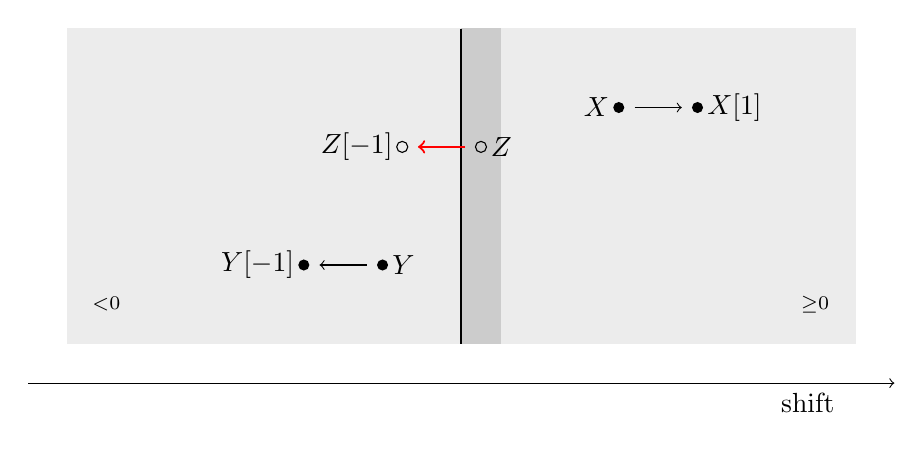
\begin{tikzpicture}%[yscale=.95]
\filldraw[gray!15] (5,-2) -- (-5,-2) -- (-5,2) -- (5, 2) -- cycle;
\filldraw[gray!40] (.5, -2) -- (0,-2) -- (0,2) -- (.5,2) -- cycle;
\draw[thick] (0,-2) -- (0,2);
\fill (2,1) circle (2pt) node[left] (X) {$X$};
\fill (-1,-1) circle (2pt) node[right] (Y) {$Y$};
\node at (4.5,-1.5) {$\C_{\geq 0}$};
\node at (-4.5,-1.5) {$\C_{<0}$};
\draw[->] (2.2,1) -- (2.8,1);
\draw[->] (-1.2,-1) -- (-1.8,-1);
\fill[xshift=1cm] (2,1) circle (2pt) node[right] (X) {$X[1]$};
\fill[xshift=-1cm] (-1,-1) circle (2pt) node[left] (Y) {$Y[-1]$};
\draw (.25,0.5) circle (2pt) node[right] {$Z$};
\draw (-.75,0.5) circle (2pt) node[left] {$Z[-1]$};
\draw[thick, ->, red] (.05,0.5) to (-.55,0.5);
\draw[->, xshift=-.5cm, yshift=-.5cm] (-5,-2) -- (6,-2) node[below, pos=.9] {\text{shift}};
\end{tikzpicture}
\caption{Heart of a $t$-structure}
\end{figure}
\end{center}
then the action of the shift functor can be represented as an horizontal shift, and the closure properties of the two classes $\C_{\geq 0},\C_{<0}$ under positive and negative shifts are a direct consequence of the shape of these areas. With these notations, an object $Z$ is in the heart of $\tee$ if it lies in a ``boundary region'', \ie if it lies in $\C_{\geq 0}$, but $Z[-1]$ lies in $\C_{<0}$.
\end{remark}
Having introduced this notation, we can rephrase the existence of the tower for $f$ as follows: given a morphism  $f\colon X\to Y$  in $\C$, for any integer $n$ and any positive integer $k$ there exists a unique factorization of $f$ 
\[
X \xto{f_{n+k}} Z_{n+k-1} \xto{f_{n+k-1}}Z_{n+k-2}\to\dots\to Z_{n+1} \xto{f_{n}} Z_{n} \xto{f_{n-1}} Y,
\]
such that
$\cofib(f_j)\in \C^\heart[j]$ for any $j=n,\dots,n+k-1$,  $\cofib(f_{n-1})\in \C_{<n}$  and $\cofib(f_{n+k})\in \C_{\geq n+k}$. 


The content of this statement becomes more interesting when $\C$ is \emph{bounded} with respect to the $t$-structure $\tee$ (see Definition \refbf{std.endocardium}). If $\C$ is bounded, then the $(\E_n,\M_n)$-factorizations of an initial morphism $0\to Y$ are trivial (see Definition \refbf{std.endocardium} and the subsequent Remark) for $|n|\gg 0$. 

As an immediate consequence, the morphisms $X \xto{f_{n+k}} Z_{n+k-1}$ and $Z_{n} \xto{f_{n-1}} Y$ in the tower of $f$ associated with the chain $n<n+1<\dots<n+k-1$ are isomorphisms for $n\ll 0$ and $k \gg 0$. One notices, as it is obvious, that the class of isomorphisms in $\C$ is closed under transfinite composition this leads to the following
\begin{proposition}\label{prop.Z.Postnikov}
Let $\C$ be a stable $\infty$-category which is bounded with respect to a given $t$-structure $\tee$. 
Then for any morphism $f\colon X\to Y$  in $\C$ there exists an integer $n_0$ and a positive integer $k_0$ such that for any integer $n\leq n_0$ and any positive integer $k$ with $k\geq n_0-n+k_0$ there exists a unique factorization of $f$ 
\[
X \xto{\sim} Z_{n+k-1} \xto{f_{n+k-1}}Z_{n+k-2}\to\dots\to Z_{n+1} \xto{f_{n}} Z_{n} \xto{\sim} Y
\]
such that
$\cofib(f_j)\in \C^\heart[j]$ for any $j=n,\dots,n+k-1$.
\end{proposition}
\begin{remark}\label{oss.Z.Postnikov}
By uniqueness in Proposition \refbf{prop.Z.Postnikov}, one has a well defined $\Z $-factorization
\[
X=\lim(Z_j) \to\cdots \to Z_{j+1} \xto{f_{j}} Z_{j} \xto{f_{j-1}}Z_{j-1}\to \cdots\to \mathrm{colim}(Z_j)=Y
\]
with 
with $j$ ranging over the integers, $\cofib(f_j)\in \C^\heart[j]$ for any $j\in \Z $ and with $f_m$ being an isomorphism for $|j|\gg 0$. We will refer to this factorization as the \emph{$\Z $-tower} of $f$. Notice how the boundedness of $\C$ has played an essential role: when $\C$ is not bounded, one still has towers for any finite ascending chain, but in general they do not stabilize.
\end{remark}
\begin{remark}\label{oss.for.Heart.to.t}
Since we know that the tower of an initial morphism is its $k$-fold $(\E_j,\M_j)$-factorization, we see that in a stable $\infty$-category $\C$ which is bounded with respect to a $t$-structure $\tee=(\C_{\geq 0},\C_{<0})$ the $\Z $-tower of $0\to Y$,
\[
0=\lim(Y_j) \to\cdots \to Y_{j+1} \xto{f_{j}} Y_{j} \xto{f_{j-1}}Y_{j-1}\to \cdots\to \mathrm{colim}(Y_j)=Y
\]
is such that $f_j\in \E_j\cap\M_{j+1}$ for any $j\in \Z $. It follows that an object $Y$ is in $\C_{\geq 0}$ if and only if the $\Z $-tower of $0\to Y$
satisfies $\cofib(f_j)=0$ for any $j< 0$, while $Y$ is in $\C_{<0}$ if and only if  $\cofib(f_j)=0$ for any $j\geq 0$.
\end{remark}
\subsection{Abelianity of the heart.}
In the following section we present a complete proof, in the stable setting, of the fact that the heart of a $t$-structure, as defined in \cite[Def. \textbf{1.2.1.11}]{LurieHA}, is an abelian $\infty$-category. 

In other words, $\C^\heart$ is homotopy equivalent to its homotopy category $h\C^\heart$, which is an abelian category; this is the higher-categorical counterpart of a classical result, first proved in \cite[Thm. \textbf{1.3.6}]{BBDPervers}, 
which 
only relies on properties stated in terms of normal torsion theories in a stable $\infty$-category. We begin with the following
\begin{definition}[Abelian $\infty$-category]\label{df:abelinfty}
An \emph{abelian $\infty$-category} is a quasicategory $\cate{A}$ such that
\begin{enumerate}
\item the hom space $\cate{A}(X,Y)$ is a homotopically discrete infinite loop space for any $X, Y$, \ie, there exists an infinite sequence of $\infty$-groupoids $Z_0, Z_1,Z_2,\dots$, with $Z_0\cong \C(X,Y)$ and homotopy equivalences $Z_i\cong \Omega Z_{i+1}$ for any $i\geq 0$, such that $\pi_n Z_0=0$ for any $n\geq 1$;
\item $\cate{A}$ has a zero object, (homotopy) kernels, cokernels and biproducts;
\item for any morphism $f$ in $\cate{A}$, the natural morphism from the \emph{coimage} of $f$ to the \emph{image} (see Definition \refbf{imcoim}) of $f$ is an equivalence.
\end{enumerate}
\end{definition}
\begin{remark}
Axiom (i) is the homotopically-correct version of $\cate{A}(X,Y)$ being an abelian group. For instance, if the abelian group is $\Z $, then the corresponding homotopy discrete space is the Eilenberg-Mac Lane spectrum $\Z ,K(\Z ,1), K(\Z ,2),\dots$. The homotopy category of such an $\cate{A}$ is an abelian category in the classical sense (note that $\cate{A}(X,Y)$ being homotopically discrete is necessary in order that kernels and cokernels in $\cate{A}$ induce kernels and cokernels in $h\cate{A}$). Moreover, since the hom spaces $\cate{A}(X,Y)$ are homotopically discrete, the natural morphism $\cate{A}\to h\cate{A}$ is actually an equivalence.
\end{remark}
The rest of the section is devoted to the proof of the following result:
\begin{theorem}\label{heart.is.abelian}
The heart $\C^\heart$ of a $t$-structure $\tee$ on a stable $\infty$-category $\C$ is an abelian $\infty$-category; its homotopy category $h\C^\heart$ is the abelian category arising as the heart of the $t$-structure $h(\tee)$ on the triangulated category $h\C$.
\end{theorem}
\begin{lemma}
For any $X$ and $Y$ in $\C^\heart$, the hom space $\C^\heart(X,Y)$ is a homotopically discrete infinite loop space.
\end{lemma}
\begin{proof}
Since $\C^\heart$ is a full subcategory of $\C$, we have $\C^\heart(X,Y)=\C(X,Y)$, which is an infinite loop space since $\C$ is a stable $\infty$-category. 

So we are left to prove that $\pi_n\C(X,Y)=0$ for $n\geq 1$. Since $\pi_n\C(X,Y)=\pi_{n-1}\Omega\C(X,Y)=\pi_{n-1}\C(X,Y[-1])$, this is equivalent to showing that 
$\C(X,Y[-1])$ is contractible. Since $X$ and $Y$ are objects in $\C^\heart$, we have $X\in \C_{[0,1)}$ and $Y[-1]\in \C_{[-1,0)}$. But $\C_{[-1,0)}$ is right object-orthogonal to $\C_{[0,1)}$ (see Remark \refbf{oss.perp}), therefore $\C(X,Y[-1])$ is contractible.
\end{proof}

The subcategory $\C^\heart$ inherits the $0$ object and biproducts (in fact, all finite limits) from $\C$, so in order to prove it is is abelian we are left to prove that it has kernels and cokernels, and that the canonical morphism from the coimage to the image is an equivalence.
\begin{lemma}\label{lemma.qua.e.la}
Let $f\colon X\to Y$ be a morphism in $\C^\heart$. Then $\mathrm{fib}(f)$ is in $\C_{<1}$ and $\cofib(f)$ is in $\C_{\geq 0}$.
\end{lemma}
\begin{proof}
Since both $X\to 0$ and $Y\to 0$ are in $\M[1]$, by the 3-for-2 property also $f$ is in $\M[1]$. Since $\M[1]$ is closed for pullbacks, $\mathrm{fib}(f)\to 0$ is in $\M[1]$ and so $\mathrm{fib}(f)$ is in $\C_{<1}$. The proof for $\cofib(f)$ is completely dual.
\end{proof}
\begin{definition}
Denote by
\[
\xymatrix{
0\ar[r]^{\E}&\ker(f)\ar[r]^{\M}&\fib(f)
}
\]
the $(\E,\M)$-factorization of the morphism $0\to \fib(f)$
and by
\[
\xymatrix{
\cofib(f)\ar[r]^{\E[1]}&\coker(f)\ar[r]^-{\M[1]} &0
}
\]
the $(\E[1],\M[1])$-factorization of the morphism $\cofib(f)\to 0$. We call $S\fib(f)=\ker(f)$ and $R_{[1]}\cofib(f)=\coker(f)$ respectively the \emph{kernel} and the \emph{cokernel} of $f$ in $\C^\heart$.
\end{definition}
\begin{remark}\label{oss.miracle}
Since $\cofib(f)[-1]\cong \fib{f}$, one can equivalently define $\coker(f)$ by declaring the $(\E,\M)$-factorization of $\fib(f)\to 0$ to be $\fib(f)\xto{\E}\coker(f)[-1]\xto{\M} 0$. Similarly, one can define $\ker(f)$ by declaring the $(\E[1],\M[1])$-factorization of $0\to \cofib(f)$ to be $0\xto{\E[1]}\ker(f)[1]\xto{\M[1]} \cofib(f)$.
By normality of the factorization system we therefore have the homotopy commutative diagram 
\[
\begin{kodi}
\obj{
	0  &|(ker)| \ker(f) &[5em] |(fib)| \fib(f)\\
	&|(0')| 0 &|(coker)| \coker(f)[-1]\\
	&&|(0'')| 0 \\
};
\mor 0 {\E}:-> ker \M:-> fib \E:-> coker \M:-> 0'';
\mor ker \E:-> 0' \M:-> coker \M:-> 0'';
\end{kodi}
\]
whose square sub-diagram is a homotopy pullout.
\end{remark}
\begin{lemma}
Both $\ker(f)$ and $\coker(f)$ are in $\C^\heart$.
\end{lemma}
\begin{proof}
By construction $\ker(f)$ is in $\C_{\geq 0}$, so we only need to show that $\ker(f)$ is in $\C_{<1}$. By definition of $\ker(f)$, we have that $\ker(f)\to \fib(f)$ is in $\M$. Since $\M[-1]\subseteq \M$, we have that also $\ker(f)[-1]\to \fib(f)[-1]$ is in $\M$.
By Lemma \refbf{lemma.qua.e.la}, $\fib(f)[-1]\to 0$ is in $\M$ and so we find that also $\ker(f)[-1]\to 0$ is in $\M$. 
The proof for $\coker(f)$ is perfectly dual.
\end{proof}
By definition of $\ker(f)$ and $\coker(f)$, the defining diagram of $\fib(f)$ and $\cofib(f)$ can be enlarged as
\[
\begin{kodi}
\obj{
0 & |(ker)| \ker(f) & |(fib)| \fib(f) & X & |(01)| 0 \\
& &|(02)| 0 & Y & |(cofib)| \cofib(f) & |(coker)| \coker(f) & |(03)| 0\\	
};
\mor 0 -> ker -> fib -> X -> 01 -> cofib -> coker -> 03;
\mor fib -> 02 -> Y -> cofib;
\mor X f:-> Y;
\mor ker k_f:{bend left},-> X; \mor Y c_f:{bend right},-> coker;
\end{kodi}
\]
where $k_f$ and $c_f$ are morphisms in $\C^\heart$.
\begin{definition}\label{imcoim}
Let $f\colon X\to Y$ be a morphism in $\C^\heart$. The \emph{image} $\im(f)$ and the \emph{coimage} $\coim(f)$ of $f$ are defined as $\im(f)=\ker(c_f)$ and  $\coim(f)=\coker(k_f)$. 
\end{definition}
The following lemma shows that $\ker(f)$ does indeed have the defining property of a kernel:
\begin{lemma}\label{is.a.kernel}
The homotopy commutative diagram
\[
\xymatrix{
\ker(f)\ar[r]^{k_f}\ar[d]&X\ar[d]^{f}\\
0\ar[r]&Y}
\]
is a pullback diagram in $\C^\heart$.
\end{lemma}
\begin{proof}
A homotopy commutative diagram 
\[
\xymatrix{
K\ar[r]\ar[d]&X\ar[d]^{f}\\
0\ar[r]&Y}
\]
between objects in the heart is in particular a homotopy commutative diagram in $\C$ so it is equivalent to the datum of a morphism $k'\colon K\to \fib(f)$ in $\C$, with $K$ an object in $\C^\heart$. By the orthogonality of $(\E,\M)$, this is equivalent to a morphism $\tilde{k}\colon K\to\ker(f)$:
\[\xymatrix{
0\ar[r]\ar[d]_{\E}&\ker(f)\ar[d]^{\M}\\
K\ar[ru]^{\tilde{k}}\ar[r]_{k'}&\fib(f)
}. \qedhere 
\]
\end{proof}
There is, obviously, a dual result showing that $\coker(f)$ is indeed a cokernel.
\begin{lemma}
The homotopy commutative diagram
\[\xymatrix{
X\ar[r]\ar[d]_{f}&0\ar[d]\\
Y\ar[r]^-{c_f}&\coker(f)
}\]
is a pushout diagram in $\C^\heart$.
\end{lemma}
\begin{lemma}\label{lemma.titanic}
For $f\colon X\to Y$ a morphism in $\C$, there is a homotopy commutative diagram where all squares are homotopy pullouts:
\[
\begin{kodi}
\obj{
|(ker)| \ker(f) &|(fib)| \fib(f) & X & 0 \\
|(01)| 0 &|(coker-1)| \coker(f)[-1] & |(Z)| Z_f &|(ker1)| \ker(f)[1] &|(02)| 0 \\
& |(03)| 0 & Y & |(cofib)| \cofib(f) & |(coker)| \coker(f) \\
};
\mor ker -> fib -> X -> 0 {{\E[1]}}:-> ker1 -> 02 {{\M[1]}}:-> coker;
\mor ker {\E}:-> 01 -> coker-1 -> Z -> ker1 {{\M[1]}}:-> cofib -> coker;
\mor fib {\E}:-> coker-1 {\M}:-> 03 -> Y -> cofib;
\mor[swap] X {\E}:-> Z {{\M[1]}}:-> Y;
\mor X f:{near start},dashed,{bend left},-> Y; 
\mor ker k_f:{bend left},-> X; 
\mor[swap] Y c_F:{bend right},-> coker;
\end{kodi}\]
uniquely determining an object $Z_f\in \C^\heart$.
\end{lemma}
\begin{proof}
Define $Z_f$ as the homotopy pullout
\[
\xymatrix{
\fib(f)\ar[r]\ar[d]_{\E} \pp & X\ar[d]^{\E}\\
\coker(f)[-1]\ar[r]& Z_f}
\]
Here the vertical arrow on the right is in $\E$ since the vertical arrow on the left is in $\E$ by definition of $\coker(f)$ (see Remark \refbf{oss.miracle}) and $\E$ is preserved by pushouts. Next, paste on the left of this diagram the pullout given by Remark \refbf{oss.miracle} and build the rest of the 
diagram by taking pullbacks or pushouts. Use again Remark \refbf{oss.miracle} and the fact that $\M[1]$ is closed under pullbacks to see that $Z_f\to Y$ is in $\M[1]$. 
Finally, we have 
\[
0\xto{\E} X\xto{\E} Z_f\xto{\M[1]} Y\xto{\M[1]} 0,
\]
and so $Z_f$ is in $\C^\heart$.
\end{proof}
\begin{proposition}\label{im.iso.coim}
There is an isomorphism $\im (f)\cong\coim (f)$.\end{proposition}
\begin{proof}
By definition, $\im(f)$ and $\coim(f)$ are defined by the factorizations
\[
\xymatrix{
0\ar[r]^{\E}&\im(f)\ar[r]^{\M}&\fib(c_f)
}
\]
and
\[
\xymatrix{
\cofib(k_f)\ar[r]^{\E[1]}&\coim(f)\ar[r]^-{\M[1]} &0
}
\]
The diagram in Lemma \refbf{lemma.titanic} shows that we have $\fib(c_f)=Z_f=\cofib(k_f)$. Therefore, 
what we need to exhibit are the $(\E,\M)$ factorizations of $0\to Z_f$ and the $(\E[1],\M[1])$ factorization of $Z_f\to 0$. Since $Z_f$ is an object in $\C^\heart$, these are
\[
0\xrightarrow{\E}Z_f\xrightarrow{\mathrm{id}_{Z_f}}Z_f
\]
and 
\[
Z_f\xrightarrow{\mathrm{id}_{Z_f}}Z_f\xrightarrow{\M[1]}0,
\]
respectively, thus giving $\im(f)\cong Z_f\cong \coim(f)$.
\end{proof}
\subsection{Abelian subcategories as hearts.}
\begin{proposition}\label{to.be.repeated.verbatim}
Let $\A$ be an abelian full subcategory of a stable $\infty$-category $\C$, such that any morphism $f\colon X\to Y$  in $\C$ has a unique $\A$-weaved $\Z$-Postnikov tower. Let
$\C_{\A,\geq 0}$ be the full subcategory of $\C$ on those objects $Y$ such that  the $\A$-weaved $\Z$-Postnikov tower
\[
0 =\lim(Y_j)\to\cdots \to Y_{j+1} \xrightarrow{f_{j}} Y_{j} \xrightarrow{f_{j-1}}Y_{j-1}\to \cdots\to \mathrm{colim}(Y_j)=Y
\]
of the initial morphism $0\to Y$ is such that $\mathrm{cofib}(f_j)=0$ for any $j< 0$, and let $\C_{\A,< 0}$ be the full subcategory of $\C$ on those objects $Y$ such that $\mathrm{cofib}(f_j)=0$ for any $j\geq 0$. Then $\mathfrak{t}_{\A}=(\C_{\A,\geq 0}, \C_{\A,<0})$ is a $t$-structure on $\C$, the stable $\infty$-category $\C$ is bounded with respect to $\mathfrak{t}_{\A}$, and the heart of $\mathfrak{t}_{\A}$ is (equivalent to) $\A$.
\end{proposition}
 The proof is split in several Lemmas. We begin introducing the following
\begin{notat}
For $\mathbf{S}$ a subcategory of $\C$, we write $\langle \mathbf{S}\rangle$ for the smallest extension closed full subcategory of $\C$ containing $S$.
\end{notat}
\begin{remark}\label{extensions}
Set  $\langle \mathbf{S}\rangle_0=\mathbf{0}$,  define $\langle \mathbf{S}\rangle_1$ as the full subcategory of $\C$ generated by $\mathbf{S}$ and $\mathbf{0}$, and define inductively $\langle \mathbf{S}\rangle_n$ as the full subcategory of $\C$ on those objects $X$ which fall into a homotopy fiber sequence
\[
\xymatrix{
X_h\ar[r]\ar[d]& X\ar[d]\\
0\ar[r] &X_k
}
\]
with $h,k\geq 1$, $X_h$ in $\langle \mathbf{S}\rangle_h$, $X_k$ in $\langle \mathbf{S}\rangle_k$ and $h+k=n$. One clearly has 
\[
\langle \mathbf{S}\rangle_0\subseteq \langle \mathbf{S}\rangle_1 \subseteq \langle \mathbf{S}\rangle_2\subseteq\cdots \subseteq \langle \mathbf{S}\rangle.
\]
Moreover $\bigcup_n \langle \mathbf{S}\rangle_n$ is clearly extension closed, so that
\[
\langle \mathbf{S}\rangle =\bigcup_n \langle \mathbf{S}\rangle_n.
\] 
\end{remark}
\begin{lemma}\label{closure}
Let $\mathbf{S}_1,\mathbf{S}_2$ be two subcategories of $\C$ with $\mathbf{S}_1\perp \mathbf{S}_2$. Then $\mathbf{S}_1\perp \langle\mathbf{S}_2\rangle$ and $\langle\mathbf{S}_1\rangle\perp \mathbf{S}_2$, and so $\langle\mathbf{S}_1\rangle\perp \langle\mathbf{S}_2\rangle$
\end{lemma}
\begin{proof}
By Remark \refbf{extensions}, to prove the first statement we are reduced to show that, if $Y\in \mathbf{S}_1$ and $X\in \langle\mathbf{S}_2\rangle_n$ then $\C(Y,X)$ is contractible. We prove this by induction on $n$. For $n=0,1$ there is nothing to prove by the assumption $\mathbf{S}_1\perp \mathbf{S}_2$. For $n\geq 2$, consider a fiber sequence $X_h\to X\to X_k$ with $1\leq h,k$ and $h+k=n$ as in Remark \refbf{extensions}. Since $\C(Y,-)$ preserves homotopy fiber sequences, we get a homotopy fiber sequence of $\infty$-groupoids
\[
\xymatrix{
\C(Y,X_h)\ar[r]\ar[d]& \C(Y,X)\ar[d]\\
{*}\ar[r] &\C(Y,X_k)
}.
\]
By the inductive hypothesis both $\C(Y,X_h)$ and $\C(Y,X_k)$ are contractible, so $\C(Y,X)$ also is. The proof of the second statement is perfectly dual, due to the fact that in $\C$ every fiber sequence is also a cofiber sequence, and $\C(-,Y)$ transforms a cofiber sequence into a fiber sequence.
\end{proof}
\begin{lemma}\label{uno}
Let $\A$ be an abelian full subcategory of $\C$. Then $\langle \{\A[s]\}_{s\geq 0}\rangle\perp \langle \{\A[s]\}_{s<0}\rangle$. In particular, in the hypothesis of Proposition \refbf{to.be.repeated.verbatim} we have $\C_{\A,\geq 0}\perp \C_{\A,<0}$
\end{lemma}
\begin{proof}
By Lemma \refbf{closure}, we only need to show that $\A[s_1]\perp \A[s_2]$ whenever $s_1\geq 0> s_2$. Let $X\in \A[s_1]$ and $Y\in\A[s_2]$. Then $X=Z_1[s_1]$ and $Y=Z_2[s_2]$ for suitable $Z_1,Z_2\in \A$ and so 
\begin{align*}
\C(X,Y)&=\C(Z_1[s_1],Z_2[s_2])\cong  \C(Z_1,Z_2[s_2-s_1])\\
&\cong \Omega^{s_1-s_2}\C(Z_1,Z_2)=\Omega^{s_1-s_2}\A(Z_1,Z_2),
\end{align*}
where in the last equality we used the fact that $\A$ is full. Since $s_1-s_2>0$, the space $\Omega^{s_1-s_2}\A(Z_1,Z_2)$ is contractible by definition of abelian $\infty$-category.
Finally, in the hypothesis of Proposition \refbf{to.be.repeated.verbatim}  one clearly has $\C_{\A,< 0}\subseteq \langle \{\A[s]\}_{s<0}\rangle$ and $\C_{\A,\geq 0}\subseteq \langle \{\A[s]\}_{s\geq 0}\rangle$.
\end{proof}
\begin{lemma}\label{due}
In the hypothesis of Proposition \refbf{to.be.repeated.verbatim} every object $Y$ of $\C$ sits into a homotopy fiber sequence $Y_{\geq 0}\to Y\to Y_{<0}$ with $Y_{\geq 0}\in \C_{\A,\geq 0}$ and $Y_{< 0}\in \C_{\A,< 0}$.
\end{lemma}
\begin{proof}
Let
\[
0 =\lim(Y_j)\to\cdots \to Y_{1} \xrightarrow{f_{0}} Y_{0} \xrightarrow{f_{-1}}Y_{-1}\to \cdots\to \mathrm{colim}(Y_j)=Y
\]
be teh $\A$-weaved Postnikov tower of $0\to Y$ and consider the pullout diagram
\[
\xymatrix{
Y_0\ar[r]\ar[d]_{f_{<0}}&0\ar[d]\\
Y\ar[r]&\mathrm{cofib}(f_{<0})
}\]
together with the $\A$-weaved $\Z$-Postnikov towers
\[
0 =\lim(Y_j)\to\cdots \to Y_{1} \xrightarrow{f_{0}} Y_{0} 
\]
and
\[
Y_{0}\xrightarrow{f_{-1}}Y_{-1}\to \cdots\to \mathrm{colim}(Y_j)=Y.
\]
The first Postnikov tower shows that $Y_0\in \C_{\A,\geq 0}$ while the second Postnikov tower shows that $\mathrm{cofib}(f_{<0})\in  \C_{\A,<0}$.
\end{proof}
\begin{lemma}\label{tre}
In the hypothesis of Proposition \refbf{to.be.repeated.verbatim}, for any $\lambda\in \R$ let
$\C_{\A,\geq \lambda}$ be the full subcategory of $\C$ on those objects $Y$ such that  the $\A$-weaved $\Z$-Postnikov tower
\[
0 =\lim(Y_j)\to\cdots \to Y_{j+1} \xrightarrow{f_{j}} Y_{j} \xrightarrow{f_{j-1}}Y_{j-1}\to \cdots\to \mathrm{colim}(Y_j)=Y
\]
of the initial morphism $0\to Y$ is such that $\mathrm{cofib}(f_j)=0$ for any $j<\lambda$, and let $\C_{\A,< \lambda}$ be the full subcategory of $\C$ on those objects $Y$ such that $\mathrm{cofib}(f_j)=0$ for any $j\geq \lambda$. 
Then, for any $n\in\Z$, one has $\C_{\A,< \lambda}[n]=\C_{\A,< \lambda+n}$ and $\C_{\A,\geq \lambda}[n]=\C_{\A,\geq \lambda+n}$. In particular, $\C_{\A,<0}[-1]\subseteq \C_{\A,<0}$ and $\C_{\A,\geq 0}[1]\subseteq\C_{\A,\geq 0}$.
\end{lemma}
\begin{proof}
Since the shift functor commutes with the formation of  $\A$-weaved $\Z$-Postnikov towers, an object $Y$ lies in $\C_{\A,< \lambda}[n]$ if and only if $\mathrm{cofib}(f_{j+n}[-n])=0$ for any $j\geq \lambda$, i.e.,  if and only if $\mathrm{cofib}(f_j)=0$ for any $j\geq \lambda+n$.
The proof for $\C_{\A,\geq \lambda}[n]$ is identical.
\end{proof}
\begin{proof}[Proof of Proposition \refbf{to.be.repeated.verbatim}]
Lemmas \refbf{uno}, \refbf{due} and \refbf{tre} together show that $\mathfrak{t}_\A=(\C_{\A,\geq 0}, \C_{\A,<0})$ is a bounded $t$-structure on $\C$. To see that the heart of  $\mathfrak{t}_\A$ is $\A$ notice that an object $Y$ lies in $\C_{\A,[0,1)}$ if and only if the $\A$-weaved $\Z$-Postnikov tower
\[
0 =\lim(Y_j)\to\cdots \to Y_{j+1} \xrightarrow{f_{j}} Y_{j} \xrightarrow{f_{j-1}}Y_{j-1}\to \cdots\to \mathrm{colim}(Y_j)=Y
\]
of its initial morphism has $\mathrm{cofib}(f_j)=0$ for every $j\neq0$, and so it is of the form
\[
\cdots 0 \to 0\to \cdots \to 0\xrightarrow{f_{0}} Y \xrightarrow{\mathrm{id}_Y}Y\xrightarrow{\mathrm{id}_Y} \cdots\xrightarrow{\mathrm{id}_Y}Y\xrightarrow{\mathrm{id}_Y}\cdots,\] 
with $Y=\mathrm{cofib}(f_0)\in \A$.
\end{proof}
\begin{remark}The same reasoning used in the proof of Proposition \refbf{to.be.repeated.verbatim}, shows that $(\C_{\A,\geq \lambda}, \C_{\A,<\lambda})$ is a bounded $t$-structure on $\C$ for every $\lambda\in \R$, and that the assignment $\lambda\mapsto (\C_{\A,\geq \lambda}, \C_{\A,<\lambda})$ is a $\Z$-equivariant morphisms of posets $\R\to \textsc{ts}(\C)$, so it is a slicing of $\C$. The heart of $(\C_{\A,\geq \lambda}, \C_{\A,<\lambda})$ is $\A[\left \lceil{\lambda}\right \rceil]$, where $\left \lceil{\lambda}\right \rceil=\min\{n\in \Z\,|\, n\geq\lambda\}$.
\end{remark}
\section{Semiorthogonal decompositions.}
\setlength{\epigraphwidth}{.75\textwidth}
\epigraph{La vie c'est ce qui se décompose à tout moment; c'est une perte monotone de lumière, une dissolution insipide dans la nuit, sans sceptres, sans auréoles, sans nimbes.}{E. Cioran, \emph{Pr\'ecis de décomposition}.}
\setlength{\epigraphwidth}{\DefaultEpigraphWidth}
At the opposite end of the transitive case studied in the previous section, there is the \emph{finite case}, where $J$ is a finite totally ordered set. As we are going to show, this is another well investigated case in the literature: $J$-familes of $t$-structures with a finite $J$ capture (and slightly generalize) the notion of \emph{semiorthogonal decompositions} for the stable $\infty$-category $\C$ (see \cite{Bondal1995, Kuz} for the notion of semiorthogonal decomposition in the classical triangulated context).

To fix notations for this section, let $J=\Delta[k-1]$ be the totally ordered set on $k$ elements seen as a poset, \ie, $J=\{i_1,i_2,\dots,i_k\}$ with $i_1\leq i_2\leq\cdots\leq i_k$, and let $\tee\colon \Delta[k-1]\to \ts(\C)$ be a $\Z $-equivariant $\Delta[k-1]$-family of $t$-structures on $\C$. We also set, for any $j=1,\dots,k+1$,
\[
\mathbf{A}_j=\C_{[i_{j-i}, i_j)}
\]
where, as usual, $i_0=-\infty$ and $i_{k+1}=+\infty$. We have that any morphism $f\colon X\to Y$ in $\C$ has a unique factorization
\[
X \xto{f_{k+1}} Z_{i_k} \xto{f_k}Z_{i_{k-1}}\to\dots\to Z_{i_{2}} \xto{f_2} Z_{i_1} \xto{f_1} Y,
\]
with $\cofib(f_j)\in \mathbf{A}_j$, and $\mathbf{A}_j\subseteq \mathbf{A}_h^\perp$, for any $1\leq j <h\leq k+1$. 

What we are left to investigate are therefore the special features of the $t$-structures $\tee_{i_j}=(\C_{\geq i_j},\C_{< i_j})$ coming from the finiteness assumption on $J$.
As we noticed in Remark \refbf{rem.finite}, a $\Z $-action on a finite poset $J$ is necessarily trivial. By $\Z $-equivariancy of the map $\Delta[k-1]\to \ts(\C)$ we have therefore that all the $t$-structures $\tee_{i_j}$ are $\Z $-fixed points for the natural $\Z $-action on $ \ts(\C)$. 

Now, a rather pleasant fact is that fixed points of the $\Z$-action on $\ts(\C)$ are precisely those $t$-structures $\tee=(\C_{\ge 0}, \C_{<0})$ for which $\C_{\ge 0}$ is a stable sub-$\infty$-category of $\C$. We will make use of the following
\begin{lemma}\label{magicstable}
Let $\cate{B}$ be a full sub-$\infty$-category of the stable $\infty$-category $\C$; then, $\cate{B}$ is a stable sub-$\infty$-category of $\C$ if and only if $\cate{B}$ is closed under shifts in both directions and under pushouts in $\C$.
\end{lemma}
\begin{proof}
The ``only if'' part is trivial, so let us prove the ``if'' part.

First of all let us see that under these assumptions $\cate{B}$ is closed under fibers. This is immediate: if $f\colon X\to Y$ is an arrow in $\cate{B}$ (\ie an arrow of $\C$ between objects of $\cate{B}$, by fullness), then $f[-1]$ is again in $\cate{B}$ since $\cate{B}$ is closed with respect to the left shift. Since $\cate{B}$ is closed under pushouts in $\C$, also  $\fib(f)=\cofib(f[-1])$ is in $\cate{B}$. It remains to show how this implies that $\cate{B}$ is actually stable, \ie it is closed under all finite limits and satisfies the pullout axiom. Unwinding the assumptions on $\cate{B}$, this boils down to showing that in the square
\[
\xymatrix{
B \ar[r]\ar[d] \pb &  X\ar[d]^f \\
Y \ar[r]_g& Z
}
\]
the pullback $B$ of $f,g \in \hom(\cate{B})$ done in $\C$ is actually an object of $\cate{B}$; indeed, once this is shown, the square above will satisfy the pullout axiom in $\C$, 
so \emph{a fortiori} it will have the universal property of a pushout in $\cate{B}$. To this aim, let us consider the enlarged diagram of pullout squares in $\C$
\[
\xymatrix{
Z[-1]\ar[r]\ar[d] \ar@{}[dr]|\star & \fib(g)\ar[r]\ar[d] & 0\ar[d] \\
\fib(f)\ar[r]\ar[d] & B\ar[r]\ar[d] & X \ar[d]^f\\
0\ar[r] & Y \ar[r]_g & Z.
}
\]
The objects $Z[-1], \fib(f)$ and $\fib(g)$ lie in $\cate{B}$ by the first part of the proof, so the square $(\star)$ is in particular a pushout of morphism in $\cate{B}$; by assumption, this entails that $B\in\cate{B}$.
\end{proof}
\begin{remark}\label{oss.shifts.pullback}
Obviously, a completely dual statement can be proved in a completely dual fashion:  a full sub-$\infty$-category $\cate{B}$ of a stable $\infty$-category $\C$ is a stable sub-$\infty$-category if and only if it is closed under shifts in both directions and under pullbacks in $\C$.
\end{remark}
\begin{proposition}\label{stableare}
Let $\tee=(\C_{\geq 0},\C_{<0})$ be a $t$-structure on a stable $\infty$-category $\C$; then the following conditions are equivalent:
\begin{enumerate}
\item $\tee$ is a fixed point for the $\Z $-action on $\ts(\C)$, \ie, $\tee[1]=\tee$ (or equivalently, $\C_{\geq 1}= \C_{\geq 0}$);
\item $\C_{\geq 0}$ is a stable sub-$\infty$-category of $\C$.
\end{enumerate}
\end{proposition}
\begin{proof}
`(2) implies (1)' is obvious. Namely, if  $\C_{\ge 0}$ is a stable sub-$\infty$-category of $\C$, then it is closed under shifts in both directions. Therefore $\C_{\ge 1}=\C_{\geq 0}[1]\subseteq \C_{\ge 0}$. Since, by definition of $t$-structure, $\C_{\geq 1}\subseteq \C_{\geq 0}$, we have $\C_{\geq 1}= \C_{\geq 0}$. To prove that `(1) implies (2)', assume $\C_{\geq 1}=\C_{\geq 0}$. This means that not only $\C_{\geq 0}[1]\subseteq \C_{\geq 0}$ as for any $t$-structure, but also $\C_{\geq 0}\subseteq \C_{\geq 0}[1]$, which implies that $\C_{\geq 0}[-1]\subseteq \C_{\geq 0}$. Therefore $\C_{\geq 0}$ is closed under shifts in both directions. By Lemma \refbf{magicstable},  we then have only to show that $\C_{\geq 0}$ is closed under pushouts in $\C$ to conclude that $\C_{\geq 0}$ is a stable $\infty$-subcategory of $\C$. Consider a pushout diagram
\[
\xymatrix{
 A \ar[r]\ar[d]_h \po & B\ar[d]^k \\
 C \ar[r] & P
}
\]
in $\C$ with $A$, $B$ and $C$ in $\C_{\geq 0}$, and let $\fF=(\E,\M)$ be the normal torsion theory associated to $\tee$. Since $A$ and $C$ are in $\C_{\geq 0} = 0/\E$ we have that both $0\to A$ and $0\to C$ are in $\E$. But $\E$ has the 3-for-2 property, so also $A\to C$ is $\E$. Since $\E$ is closed for pushouts, this implies that also $B\to P$ is in $\E$. But $0\to B$ in in $\E$ since $B$ is in $\C_{\geq 0}$, and therefore also $0\to P$ is in $\E$, \ie, $P$ is in $\C_{\geq 0}$.
\end{proof}
\begin{remark}\label{dual.of.the.above}
The statement of \aprop \refbf{stableare} can easily be dualized: $\Z $-fixed points in $\ts(\C)$ as those $t$-structures $(\C_{\geq 0},\C_{<0})$ for which $\C_{<0}$ is a stable sub-$\infty$-category of $\C$, as well as those such that $\C_{<0} = \C_{<1}$.
\end{remark}
Proposition \refbf{stableare} and remark \refbf{dual.of.the.above} characterize $\Z $-fixed points on $\ts(\C)$ as the $t$-structures with stable classes $\C_{\geq 0}$ and $\C_{<0}$. By the correspondence between $t$-structures and normal factorization systems, one should expect that these should be equally characterized as the normal factorization systems  $\fF=(\E,\M)$ for which the classes $\E$ and $\M$ are ``stable on both sides'', \ie, are closed both for pullbacks and for pushouts.
\begin{theorem}\label{enactedstableare}
Let $\tee$ be a $t$-structure on a stable $\infty$-category $\C$ and let $\fF=(\E,\M)$ be the corresponding normal factorization system; then the following conditions are equivalent:
\begin{enumerate}
\item $\tee[1]=\tee$;
\item $\C_{\geq 0}$ is a stable $\infty$-category;
\item $\C_{< 0}$ is a stable $\infty$-category;
\item $\E$ is closed under pullback;
\item $\M$ is closed under pushout.
\end{enumerate}
\end{theorem}
\begin{proof}
In view of the previous results, the only implication we need to prove is that `(1) is equivalent to (4)'. Assume $\E$ is closed under pullbacks. Then for any $X$ in $\C_{\geq 0}$ we have that $0\to X$ is in $\E$, and so $X[-1]\to 0$ is in $\E$. By the Sator lemma this implies that $0\to X[-1]$ is in $\E$, \ie, that $X[-1]$ is in $\C_{\geq 0}$. This shows that $\C_{\geq 0}[-1]\subseteq \C_{\geq 0}$ and therefore that $\tee[1]= \tee$. 

Conversely, assume $\tee[1]=\tee$,
and consider a morphism $f\colon X\to Y$ in $\E$. For any morphism $B\to Y$ in $\C$
consider the diagram
\[
\xymatrix{
\mathrm{fib}(f)\ar[r]\ar[d] & A\ar[r]\ar[d] & X\ar[r]\ar[d]^{f} & 0\ar[d]\\
0 \ar[r] & B\ar[r]  & Y\ar[r]  & \cofib(f)
}
\]
where all the squares are pullouts in $\C$. Since $f$ is in $\E$ and $\E$ is closed for pushouts, also $0\to \cofib(f)$ is in $\E$. This means that $\cofib(f)$ is in $\C_{\geq 0}$ and so, since we are assuming that $\C_{\geq 0}=\C_{\geq 0}[-1]$, also $\mathrm{fib}(f)=\cofib(f)[-1]$ is in $\C_{\geq 0}$, \ie,  $0\to \mathrm{fib}(f)$ is in $\E$. By the Sator lemma, $\mathrm{fib}(f)\to 0$ is in $\E$, which is closed for pushouts, and so $A\to B$ is in $\E$.
\end{proof}
\begin{remark}\label{oss.hereditary}
In the literature, a factorization system $(\E,\M)$ for which the class $\E$ is closed for pullbacks is sometimes called an \emph{exact reflective} factorization, see, \eg, \cite{CHK}. This is equivalent to saying that the associated reflection functor is left exact (this is called a \emph{localization} in the jargon of \cite{CHK}). Dually,  one characterizes \emph{colocalizations} of a category $\C$ with an initial object as \emph{coexact coreflective} factorizations where the right class $\M$ of $\fF$ is closed under pushouts.  Therefore, in the stable $\infty$-case, we see that a $\Z $-fixed point in $\ts(\C)$ is a $t$-structure $(\C_{\geq 0},\C_{<0})$ such that the truncation functors $\tau_{\ge 0}\colon \C\to \C_{\ge 0}$ and $\tau_{<0}\colon \C\to \C_{<0}$ respectively form a colocalizations and a localization of $\C$. In the terminology of \cite{Beligiannisreiten} we therefore find that in the stable $\infty$-case $\Z $-fixed point in $\ts(\C)$ correspond to \emph{hereditary torsion pairs} on $\C$. Since we have seen that for a $\Z $-fixed point in $\ts(\C)$ both $\C_{\geq 0}$ and $\C_{<0}$ are stable $\infty$-categories, this result could be deduced also from \cite[Prop. \textbf{1.1.4.1}]{LurieHA}: a left (resp., right) exact functor between stable $\infty$-categories is also right (resp., left) exact.
 \end{remark}
We can now precisely relate semiorthogonal decompositions in a stable $\infty$-category $\C$ to $\Delta[k-1]$-families of $t$-structures on $\C$. The only thing we still need is the following definition, which is an immediate adaptation to the stable setting of the classical definition given for triangulated categories (see, \eg, \cite{Bondal1995, Kuz} ).
\begin{definition}
Let $\C$ be a stable $\infty$-category. A \emph{semiorthogonal decomposition} with $k$ classes on $\C$ is the datum of $k+1$ stable $\infty$-subcategories $\mathbf{A}_1$, $\mathbf{A}_2$,\dots, $\mathbf{A}_{k+1}$ of $\C$ such that
\begin{enumerate}
\item one has $\mathbf{A}_i\subseteq \mathbf{A}_j^\perp$ for $i<j$ (semiorthogonality);
\item for any object $Y$ in $\C$ there exists a unique $\{\mathbf{A}_i\}$-weaved tower, \ie, a factorization of the initial morphism $0\to Y$ as 
\[
0 =Y_0\to\cdots \to Y_{j+1} \xto{f_{j}} Y_{j} \xto{f_{j-1}}Y_{j-1}\to \cdots\to Y_{k+1}=Y
\]
with $\cofib(f_j)\in \mathbf{A}_j$ for any $j=1,\dots, k+1$. 
\end{enumerate} 
\end{definition}
\begin{remark}
Since $\{\mathbf{A}_i\}$-weaved Postnikow towers are preserved by pullouts, one can equivalently require that any morphism $f\colon X\to Y$ in $\C$ has a unique factorization of the form 
\[
X =Z_0\to\cdots \to Z_{j+1} \xto{f_{j}} Z_{j} \xto{f_{j-1}}Z_{j-1}\to \cdots\to Z_{k+1}=Y
\]
with $\cofib(f_j)\in \mathbf{A}_j$ for any $j=1,\dots, k+1$. 
\end{remark} 
\begin{theorem}\label{what.s.semiortho}
Let $\C$ be a stable $\infty$-category. Then the datum of a semiorthogonal decompositions with $k$ classes on $\C$ is equivalent to the datum of a $\Z $-equivariant $\Delta[k-1]$-family of $t$-structures on $\C$
\end{theorem}
\begin{proof}
Let us start with a $\Z $-equivariant $\Delta[k-1]$-family of $t$-structures $\tee$, and write $i_1<i_2<\cdots<i_k$ for the elements of $\Delta[k-1]$ and $\tee_{i_j}=(\C_{\geq i_j},\C_{<i_j})$ for the corresponding $t$-structures on $\C$. Then, setting $\mathbf{A}_j=\C_{[i_{j-1}, i_j)}$ we have semiorthogonality between the $\mathbf{A}_j$'s and the existence of $\{\mathbf{A}_j\}$-weaved Postnikow towers by the general argument recalled at the beginning of this section. So we are only left to prove that the subcategories $\mathbf{A}_j$ are stable. This is immediate: by Theorem \refbf{enactedstableare} both the sub-$\infty$-categories $\C_{\geq i_{j-1}}$ and $\C_{<i_j}$ are stable, and so also their intersection is stable (see, \cite{LurieHA}). Vice versa, if we start with a semiorthogonal decomposition, then repeating verbatim the argument in the proof of Proposition \refbf{to.be.repeated.verbatim} one defines 
a $\Z $-equivariant $\Delta[k-1]$-family of $t$-structures on $\C$.
\end{proof}
\begin{remark}By Remark \refbf{oss.hereditary}, we recover in the stable $\infty$-setting the well known fact (see \cite[\textbf{IV.4}]{Beligiannisreiten}) that semiorthogonal decompositions with a single class correspond to \emph{hereditary torsion pairs} on the category.
\end{remark}
\section{Tilting theory}
\epigraph{Quando si vuole uccidere un uomo bisogna colpirlo al cuore, e un Winchester è l'arma più adatta.}{Ramón Rojo}
Let us first recall (\adef \refbf{df:abelinfty}) that an abelian $\infty$\hyp{}category is an $\infty$\hyp{}category with biproducts, kernels and cokernels, and image\hyp{}factorization which is in addition \emph{homotopically discrete}.

It is not surprising that the language of abelian $\infty$\hyp{}categories is rich enough to interpret the notion of normal torsion theory:\footnote{This is the context where historically torsion theories were introduced \cite{dickson1966torsion}; in some sense, stable categories are ontologically more primitive since ``all'' abelian categories arise as hearts of suitable $t$\hyp{}structures.} to be more precise, we can define a (normal) torsion theory on an abelian $\infty$\hyp{}category $\A$, only paying attention to the fact that the stable setting endows the definition with several useful autodualities (like the equivalence between semiexact and normal torsion theories in \cite{Fiorenza2014}) false in the abelian setting.

Start with the following example: let $\C = \cate{D}(\A)$ be the derived $\infty$\hyp{}category of an abelian category $\A$; it is interesting to ask which (factorization functors of) normal torsion theories $\tee_\C$ on $\D(\A)$ factor through $\A = \D(\A)^\heart \subset \D(\A)$; this means that
\begin{enumerate}
\item we have (mild) co\fshyp{}completeness conditions on $\A$, that amount to the existence in $\A$ of finite co\fshyp{}limits;
\item the reflection $R$ and coreflection $S$ of $\tee_\C$ factor as follows:
\[
\xymatrix{
	\C^\heart \ar[rr]^{S|_{\C^\heart}}\ar@{.>}[dr]_{\hat S} && 0/ \E \\
	 & 0/\E \cap \C^\heart \ar[ur]
}\qquad
\xymatrix{
	\C^\heart \ar[rr]^{R|_{\C^\heart}}\ar@{.>}[dr]_{\hat R}  && \M/0 \\
	 & \M/0 \cap \C^\heart \ar[ur]
}
\]
\end{enumerate} 
This informal definition is needed to cope with a torsio\hyp{}centric reformulation of \emph{tilting theory}. Our aim here is not to delve into the details of such an intricate and vast topic, but only to skim the surface of it: indeed, 
at the level of generality we are interested in, \emph{tilting} of a $t$\hyp{}structure $\tee$ is a device to produce another $t$\hyp{}structure out of $\tee$ and a (normal) torsion theory on the heart $\C^{\heart, \tee}$; the $t$\hyp{}structure on $\C$ are acted by (normal) torsion theories on their hearts.
\begin{definition}
Let $\C$ be a stable $\infty$\hyp{}category, $\fF = (\E, \M)$ a normal torsion theory on $\C$ and $\mathbb{T} = (\mathcal{X}, \mathcal{Y})$ a torsion theory on the heart $\C^{\heart, \tee}$. We define the two classes
\begin{align}
\E \tilt \mathcal{X} &= \{f\in \hom(\C)\mid f\in \E [-1],\; h_\tee(f)\in \mathcal{X}\}\notag\\
\M \tilt \mathcal{Y} &= \{g\in \hom(\C)\mid g\in \M [1], \; h_\tee(g)\in \mathcal{Y}\},\footnotemark
\end{align}
\footnotetext{The symbol $\tilt$ (pron. \emph{retort}) recalls the alchemical token for an alembic; here the term hints at the double meaning of the word retort.}
where $h_\tee\colon \C \to \C^{\heart,\tee}$ is the canonical functor of projection to the heart. These two classes define a new normal torsion theory $\tee \tilt \mathbb{T}$ on $\C$, called the \emph{tilting} of $\tee$ by $\bT$.
\end{definition}
\begin{remark}
The idea behind the definition of tilting is to have a way to factor morphisms ``until the upper half\hyp{}plane'', and below the horizontal line $Y=1$;\footnote{The $Y$ axis is oriented downwards: see Figure \refbf{tilting.fac} below.} specifying a (normal) torsion theory on $\C^{\heart, \tee}$ amounts to specifying a factorization on the objects of the strip $[0,1)$.
\end{remark}
\begin{proposition}
Let $\bT$ be a (normal) torsion theory on $\C^{\heart,\tee}$, and let $\mathbb{S}$ another (normal) torsion theory on $\C^{\heart, \tee\;\tilt\; \bT}$.  Now, the tilting operation ``behaves like an action'', namely
\begin{itemize}
\item $(\tee\tilt \bT)\tilt \mathbb{S} = \tee \tilt (\bT \star \mathbb{S})$, for an operation $\star$ between (normal) torsion theories on the heart; 
\item $\tee \tilt \bT_{\tee} = \tee$, if $\bT_\tee$ is the factorization system induced by $\tee$ on its heart.
\end{itemize}
\end{proposition}
\begin{definition}[Compatible $t$\hyp{}structures]
Let $\fF, \fF'$ be two $t$\hyp{}structures on the stable $\infty$\hyp{}category $\C$; then $\fF'$ is \emph{compatible with $\fF$} (or \emph{$\fF$\hyp{}compatible}) if the $\fF'$\hyp{}factorization of every object $X\in\C^{\heart,\tee}$ belongs again to $\C^{\heart,\tee}$.
\end{definition}
In view of the definition of the heart functor $h_\tee\colon \C \to \C^{\heart,\tee}$ as $X\mapsto R_1 S_0 X$, and since an object $A\in\C$ lies in $\C^{\heart,\tee}$ if and only if $h_\tee A \cong A$, we have that $\fF'$ is $\fF$\hyp{}compatible if and only if its coreflection\fshyp{}reflection pair $(S', R')$ is such that 
\[
R_1 S_0 S' = S'; \qquad\qquad R_1 S_0 R'  = R'.
\]
\begin{remark}
Let $J$ be a $\Z$\hyp{}poset and $\tee\colon J\to \ts(\C)$ a $J$\hyp{}slicing on $\C$; let $\bar \jmath$ a specified element of $J$ and $\tee_{\bar\jmath} = (\E_{\bar\jmath}, \M_{\bar\jmath})$ its image under $\tee$; then, every $\tee_j$ such that $\tee_{\bar\jmath+1}\preceq \tee_j \preceq \tee_{\bar\jmath}$ is $\tee_{\bar\jmath}$\hyp{}compatible.
\end{remark}
\begin{proposition}
Given $\fF, \fF'$ compatible $t$\hyp{}structures on $\C$, $\fF'$ induces a normal torsion theory on the heart $\C^{\heart, \tee}$, denoted $\fF'|_\tee$, and $\fF \tilt (\fF'|_\tee) = \fF'$.
\end{proposition}
% \begin{proof}
% \fare
% \end{proof}
\begin{proposition}
There is a bijective correspondence between tiltings of $\fF$ by (normal) torsion theories on $\C^{\heart, \tee}$ and $\fF$\hyp{}compatible normal torsion theories on $\C$.
\end{proposition}
The situation is best depicted in the following picture giving the factorization rule; this also yields orthogonality of the two classes so determined.
\begin{figure}[h]
\begin{kodi}
\begin{scope}
\clip (0,-3cm) rectangle (10,3cm);
\draw[line width=6cm,lightgray] (0,0) -- (10,0);
\draw[line width=2.5cm,gray!90!white] (0,0) -- (10,0);
\end{scope}
\draw[thick,yshift=1.25cm] (0,0) -- (10,0) node[right] {$0$};
\draw (10,-1.25) node[right] {$1$};
\node[above] (X) at (7.5,2.5) {$X$};
\node[below] (Y) at (7.5,-2.5) {$Y$};
\node[left,shape=circle,fill=gray!90!white,inner sep=.2em,outer sep=.2em]  (A) at (1.5,1.25) {$A$};
\node[right] (B) at (4.5,0) {$B$};
\node[left,shape=circle,fill=gray!90!white,inner sep=.2em,outer sep=.2em] (C) at (2.5,-1.25) {$C$};
\mor X f:{bend left},-> Y;
\draw[->] (X) -- (A);
\draw[->] (A) -- (B);
\draw[->] (B) -- (C);
\draw[->] (C) -- (Y);
\draw[->,dashed,thick] (X.210) to [bend right] (B);
\draw[->,dashed,thick] (B) to [bend right] (Y.140);
\end{kodi}
\caption{Tilting factorization of $f$.}
\label{tilting.fac}
\end{figure}
Even if the result can also be obtained from a direct argument, as a consequence of the following general fact about ternary FS:
\begin{lemma}[Tilting of factorizations]\label{tilted.FS}
Let $\tee\colon \Z\to \ts(\C)$ be a $\Z$\hyp{}family of normal torsion theories on a stable $\infty$\hyp{}category $\C$, having values $\tee_i = (\E_i, \M_i)$ for $i\in\Z$ (here, we will only consider the values $\tee_0, \tee_1 = \tee_0[1]$); let $(\LL,\mathcal{R})$ be a torsion theory on the heart $\C^\heart = \C_{[0,1)}$ such that $\E_1\subseteq \LL \subseteq \E_0$ (equivalently, $\M_0 \subseteq \R \subseteq \M_1$). Then, the factorization $(e_{\mintilt},m_{\mintilt})$
\[
\begin{kodi}
\obj{
X & A && B & Y \\
&& S &&\\	
};
\mor X e_1:-> A {e_0 \cdot m_1}:-> B m_0:-> Y;
\mor[swap] A l:-> S r:-> B;
\mor[dashed, bend right,swap] X {e_{\mintilt}}:-> S {m_{\mintilt}}:-> Y;
\end{kodi}
\]
of a morphism $f\colon X\to Y$ in $\C$, obtained from the synergy of the ternary factorization induced by $\tee_0 \preceq \tee_1$, plus the $(\mathcal{L},\mathcal{R})$\hyp{}factorization of its middle part $A\to B \in \E_0\cap \M_1$, defines a factorization system on $\C$, called the \emph{tilting} of $\tee$ (confused with its $0$\hyp{}value $\tee_0$, in view of Remark \refbf{trivial.but.useful2}) by $(\LL, \fR)$, and denoted $\tee\tilt (\LL,\fR)$.
\end{lemma}
\begin{proof}
We have to show that the rule outlined above constitutes a factorization system; the stretagy is to summon \cite[\athm \textbf{A}]{Korostenski199357} again (see the proof of the ``Rosetta stone'' in \cite{Fiorenza2014}).

Now, this allows us to conclude since given a lifting problem
\[
\begin{kodi}
\obj{
X & A \\
Y & B \\	
Z & C \\
};
\mor X u:-> A r:-> B m_0:-> C;
\mor[swap] X e_1:-> Y l:-> Z v:-> C;
\mor[dashed] Y x:-> C;
\mor[dashed] Y y:-> A;
\mor[dashed] Z z:-> A;
\end{kodi}
\]
the arrows $x,y,z$ obtained respectively as composition $v\circ l$, and as solutions to suitable lifting problems, give the desired orthogonality.
\end{proof}
\bibliography{allofthem}{}
\bibliographystyle{amsalpha}
\hrulefill 
\begin{center}
\boxed{
\begin{minipage}{.5\textwidth}
Todo:

$\bullet$ mettere a posto le crossref 
(che al momento puntano alla tesi)


\end{minipage}}
\end{center}
\end{document}
